\chapter{抗原}
\begin{framed}
\noindent\textbf{【知识体系】}
\begin{center}
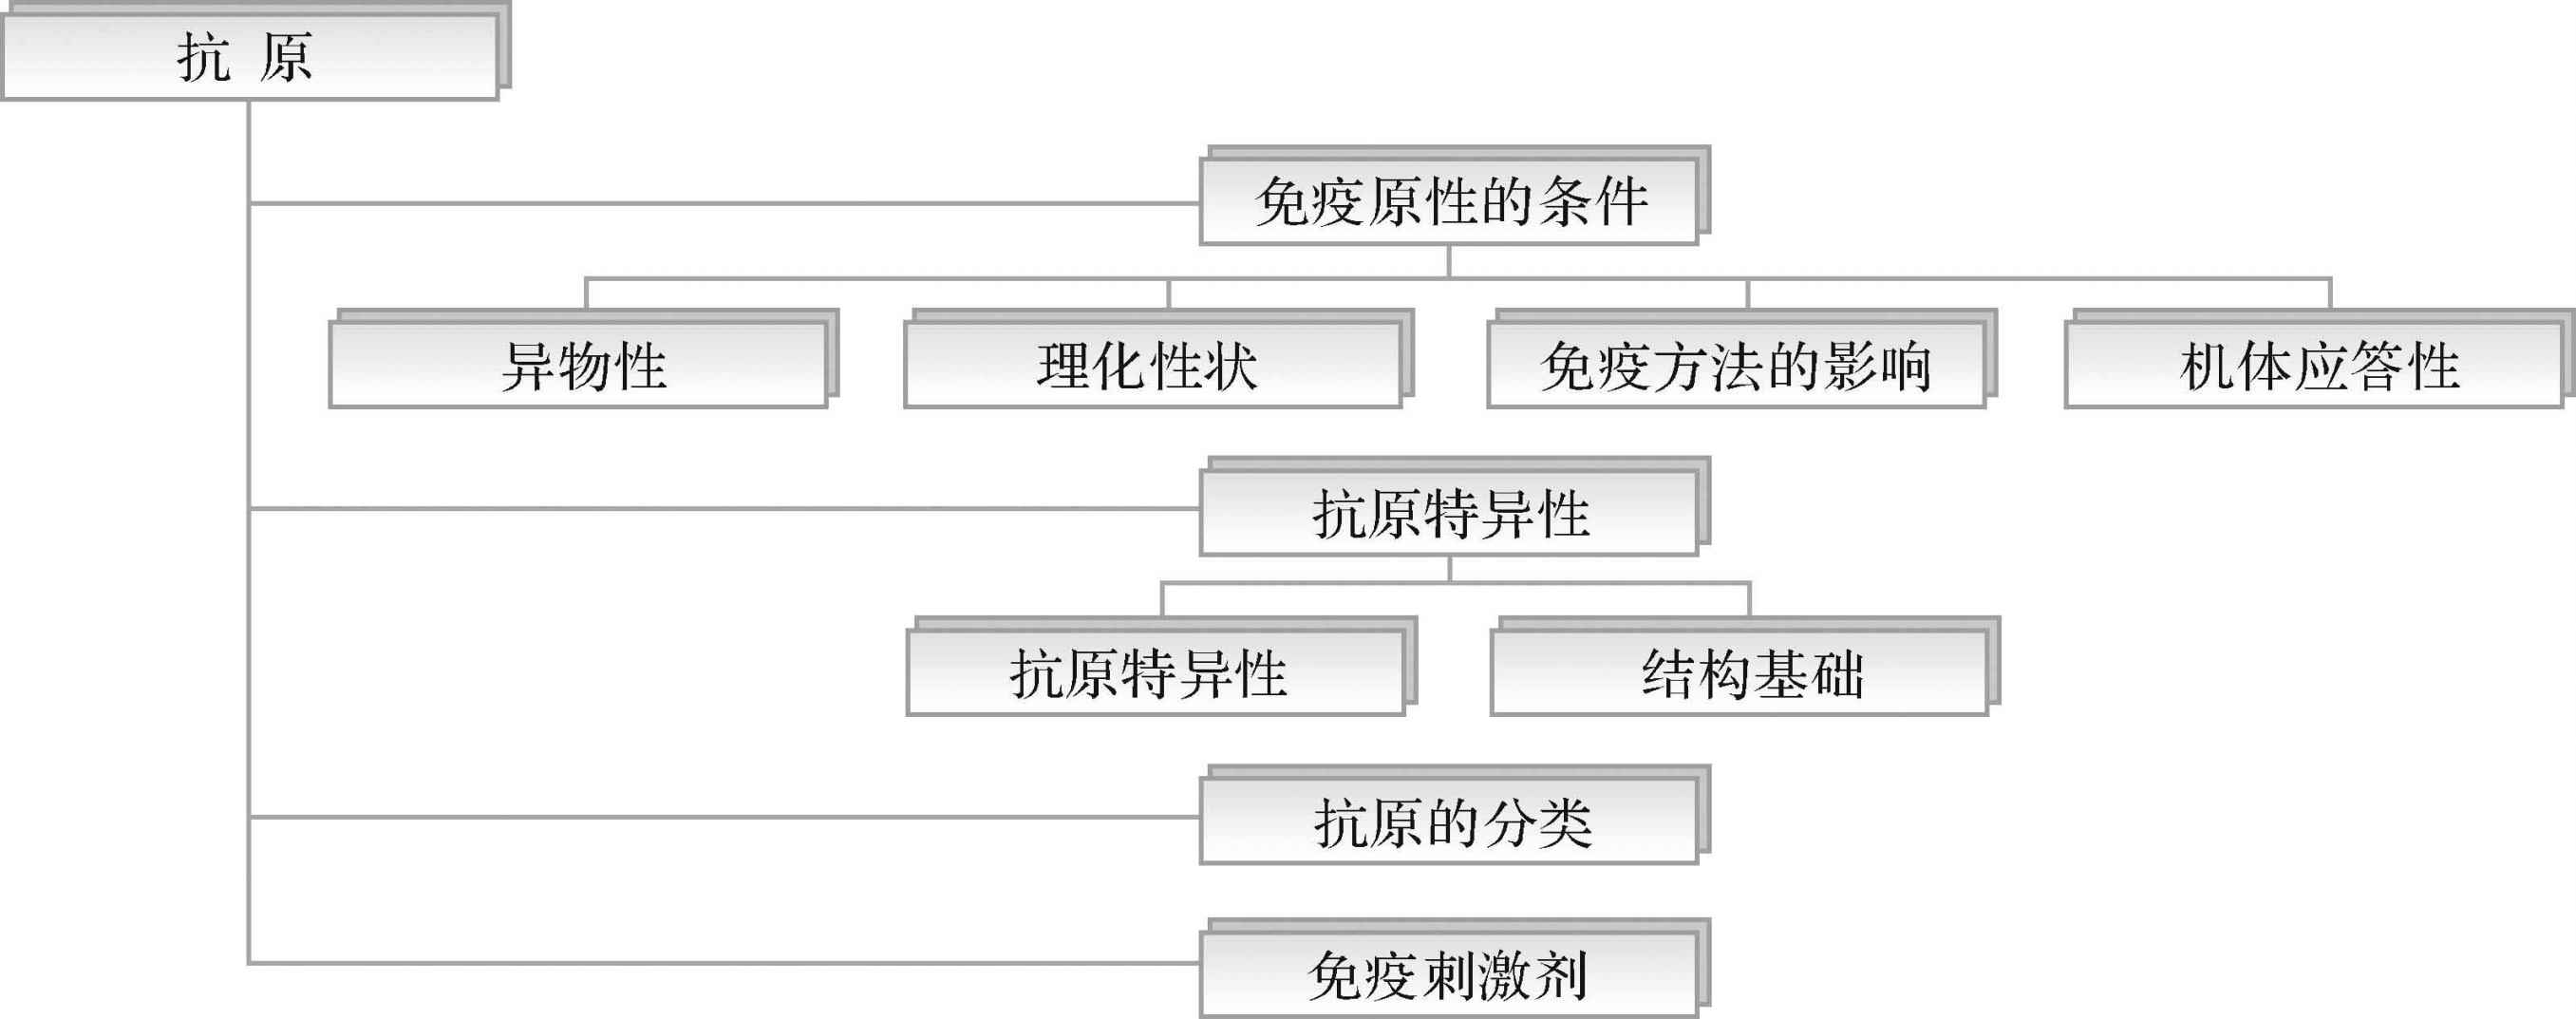
\includegraphics{./images/Image00049.jpg}
\end{center}
\noindent\textbf{【课前思考】}

哪些物质进入机体(或体内病变的成分)能被机体识别并排除?为什么静脉注射生理盐水、食物进入机体没有异样,而将蛋白质(如蛋清)注射入体内则引起机体反应?机体为什么能识别有细微差别的异物?这细微差别是什么?

\noindent\textbf{【本章重点】}

1.决定免疫原性的条件;

2.抗原特异性与抗原决定簇的关系;

3.TD抗原,TI抗原、免疫佐剂的概念。

\noindent\textbf{【教学目标】}

1.掌握决定免疫原性的条件;

2.掌握抗原的特异性与抗原决定簇的关系;

3.熟悉抗原的分类;

4.了解免疫佐剂的种类、作用及应用。
\end{framed}

抗原(antigen)是指那些能够诱导机体免疫系统产生免疫应答,又能与相应抗体或致敏淋巴细胞在体内外发生特异性反应的物质。因此,抗原具有两个重要特性:

(1)免疫原性(immunogenicity):即抗原能够刺激机体产生抗体或致敏淋巴细胞的能力;

(2)免疫反应性(immunoreactivity)或反应原性:即抗原能够与其所诱生的抗体或致敏淋巴细胞特异性结合的能力。

具备上述两种特性的物质为完全抗原,一般而言,具有免疫原性的物质均具免疫反应性,即均属完全抗原,如:微生物、异种蛋白;仅具备免疫反应性(即抗原性)的物质被称为半抗原(hapten),如:某些多糖、类脂、药物。半抗原与载体蛋白结合成为半抗原---载体复合物(完全抗原)。半抗原可作为抗原决定基研究其特异性。

\section{决定免疫原性的条件}

免疫原性是判断一种物质是否为抗原的关键。免疫原性主要取决于物质本身的性质及其与机体的应答性。


\subsection{异物性}

异物性的程度取决于其与机体的亲缘关系:亲缘关系(即种属关系)越远,则异物性越强,即免疫原性越强。例如:鸡卵蛋白对鸭是弱抗原,对哺乳动物则是强抗原;灵长类(猴或猩猩)的组织成分对人是弱抗原,而病原微生物对人则多为强抗原;临床上选择同种器官移植物时,供者与受者的亲缘关系越近(例如有血缘关系),则排斥反应的程度越轻。

1.异种物质:如微生物及其代谢产物、异种血清蛋白、组织细胞等。

2.同种异体物质:同种不同个体间,如血型。

3.改变和隐蔽的自身物质:在外伤、感染、电离辐射等作用下,结构改变,成为“非己”抗原,产生应答。


\subsection{理化性状}

1.大分子物质:天然抗原多为大分子有机物,多数蛋白质为良好的抗原,多糖及多肽也具一定的免疫原性,此与其化学性质有关。

分子量>10000 ------免疫原性好,如:异种蛋白、多糖。

10000>分子量>4000------弱免疫原性。

分子量<4000------不具有免疫原性,如:小分子多肽、核酸。

大分子物质成为抗原的原因:

(1)表面抗原决定簇多。

(2)组成复杂,结构稳定,不易被破坏和清除。在体内停留的时间长,可持续刺激。

分子量并非决定免疫原性的唯一和绝对因素,免疫原性物质还须具备复杂的化学组成与特殊的化学基团。例如:简单重复的有机大分子不具免疫原性(如磺化聚苯乙烯);明胶的分子量逾100kD,但其仅由直链氨基酸组成,故免疫原性很弱;胰岛素分子量仅为5.7kD,但其序列中含芳香族氨基酸,故具免疫原性。

化学性质相同的抗原物质可因其物理性状不同而影响免疫原性。例如:颗粒抗原的免疫原性强于可溶性抗原;多聚体的免疫原性强于单体。

2.化学结构:结构越复杂,其免疫原性越强。


\subsection{免疫方法的影响}

1.抗原的剂量太低或太高都不行,纯化的抗原每次要达到ug或mg水平。

2.免疫途径:同一物质经不同途径进入机体,其刺激免疫系统产生应答的强度各异,依次为皮内>皮下>肌肉>腹腔(仅限于动物)
>静脉。一般而言,抗原物质从非经口途径进入机体可显示较强的免疫原性。经口服给予的蛋白质类抗原物质(如鸡蛋、牛奶等),可在消化道内被降解为氨基酸,从而丧失其免疫原性。


\subsection{机体应答性}

1.同种但不同品系的动物,其对同一抗原产生应答的强度或性质各异。如:纯化多糖在人、鼠是强抗原,在豚鼠是弱抗原。

2.同一品系有个体差异:如:疫苗对有的人有保护力,对有的人是弱保护力。

\section{抗原特异性}


\subsection{抗原特异性}

抗原特异性指抗原诱导机体产生应答及与应答产物发生反应所显示的专一性。特定抗原只能刺激机体产生特异性抗体或致敏淋巴细胞,且仅能与该特异性抗体或淋巴细胞结合并相互作用。例如:接种破伤风类毒素仅能诱导机体产生针对该毒素的抗体,且这种抗体仅与破伤风毒素结合,而不与白喉毒素结合;接种乙肝疫苗仅能预防乙肝,而不能预防痢疾。


\subsection{决定抗原特异性的分子结构基础}

\begin{figure}[!htbp]
 \centering
 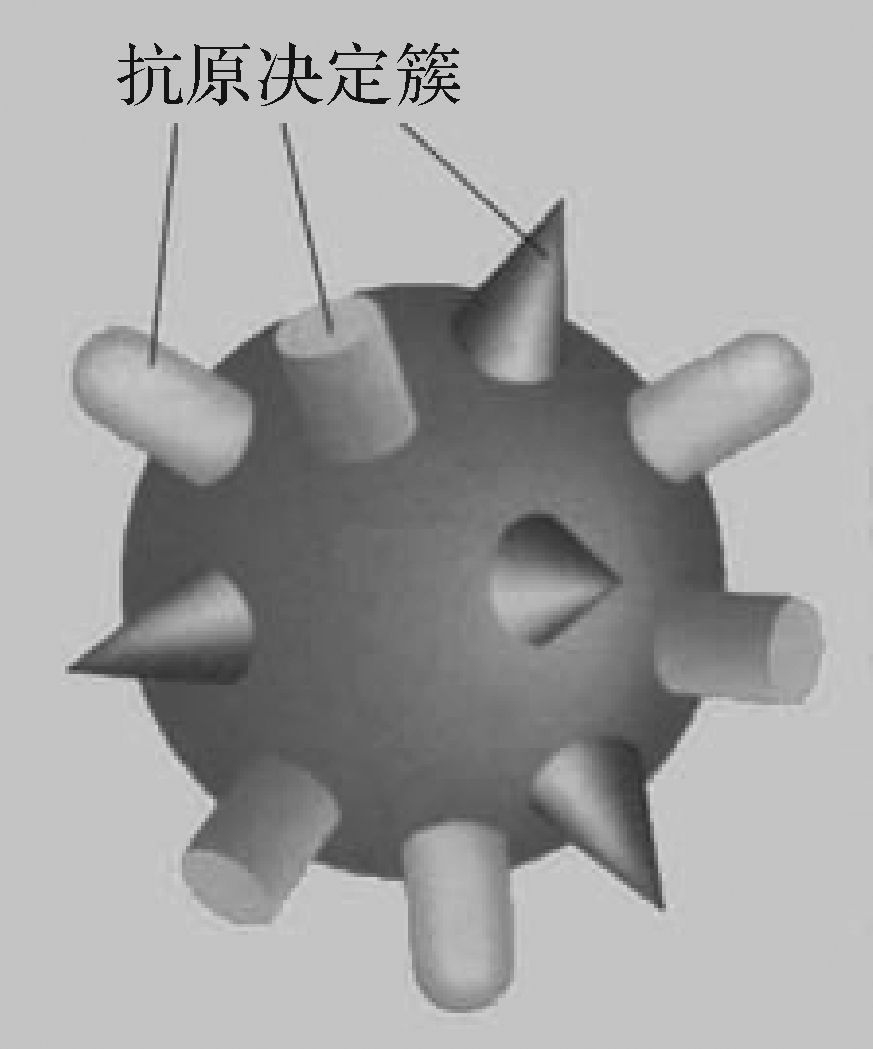
\includegraphics{./images/Image00050.jpg}
 \captionsetup{justification=centering}
 \caption{抗原决定簇示意图}
 \label{fig3-1}
  \end{figure}

1.抗原决定簇:决定抗原特异性的基本结构或化学基团称为表位(epitope),亦称为抗原决定簇(Antigen
Determinant
AD)(图\ref{fig3-1})。通常5~15个氨基酸残基、5~7个多糖残基或核苷酸即可构成一个表位。表位结构的性质与位置可影响抗原的特异性。

抗原的特异性决定于抗原决定簇的性质、氨基酸或碳水化合物的种类、序列及空间立体构型。

2.抗原价:抗原分子表面能够与抗体结合的表位数量称为抗原价(图\ref{fig3-2}),完全抗原一般均为多价抗原。如:牛血清白蛋白有18个AD。有的只有一个AD即单价抗原(半抗原),如:肺炎球菌荚膜多糖水解产物。

\begin{figure}[!htbp]
 \centering
 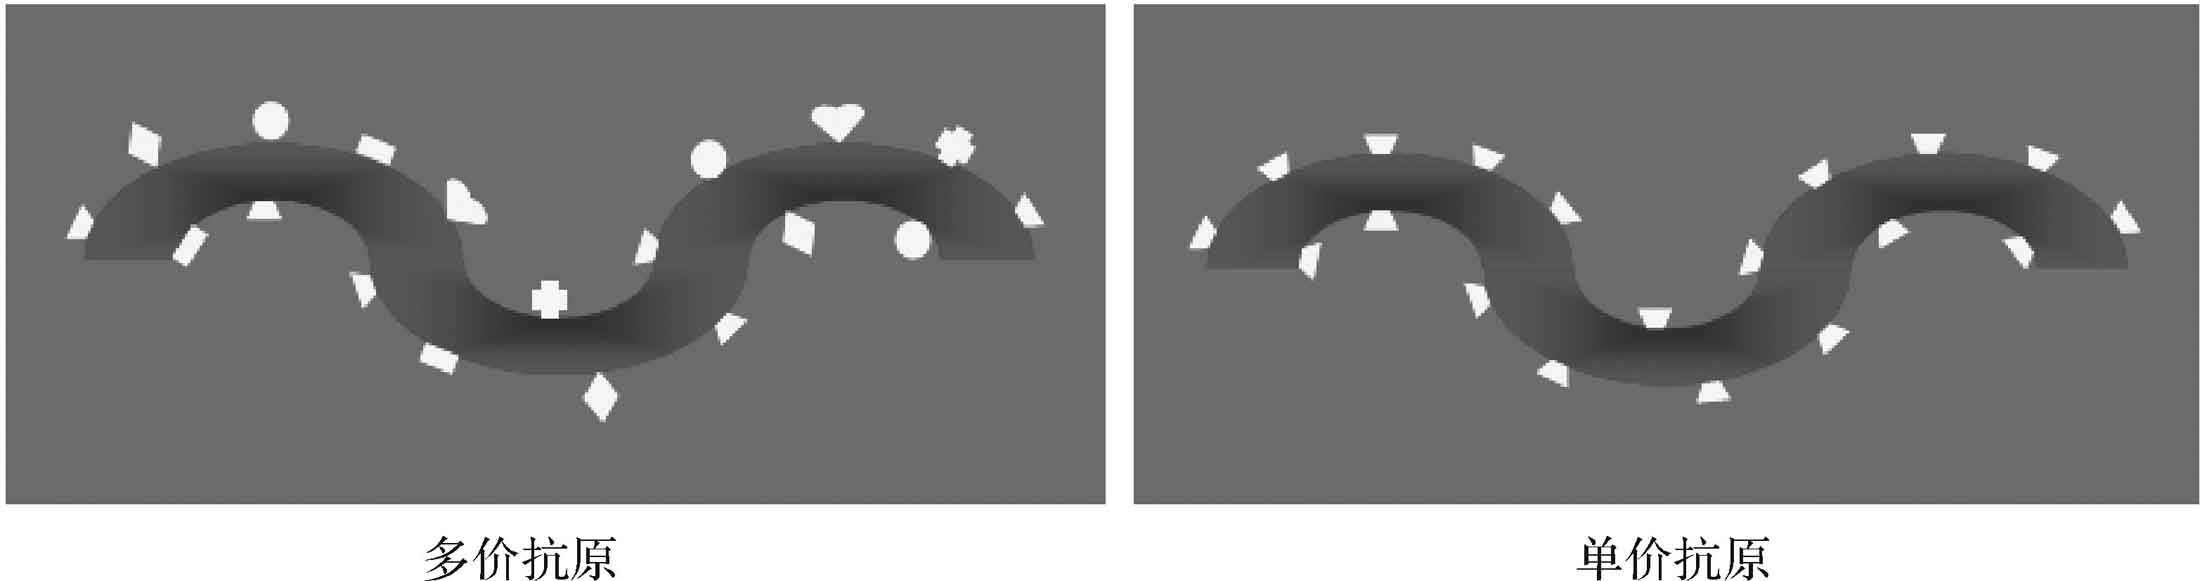
\includegraphics[width=.6\textwidth]{./images/Image00051.jpg}
 \captionsetup{justification=centering}
 \caption{抗原价}
 \label{fig3-2}
  \end{figure}

3.功能决定簇和隐蔽决定簇:

功能性决定簇:暴露在抗原分子表面,启动参与应答有决定意义。

隐蔽决定簇:在抗原的内部,无法触发免疫应答,只有经理化处理暴露后,才起作用。

4.表位结构的性质与位置可影响抗原的特异性。抗原决定簇性质对抗原特异性的影响:对苯胺、对氨苯甲酸、对氨苯磺酸和对氨苯砷酸4种半抗原分子间仅存在一个有机酸基团的差异,分别与载体结合后(成为完全抗原)可诱导机体产生相应抗体,后者仅能与对应的半抗原结合(图\ref{fig3-3})。

\begin{figure}[!htbp]
 \centering
 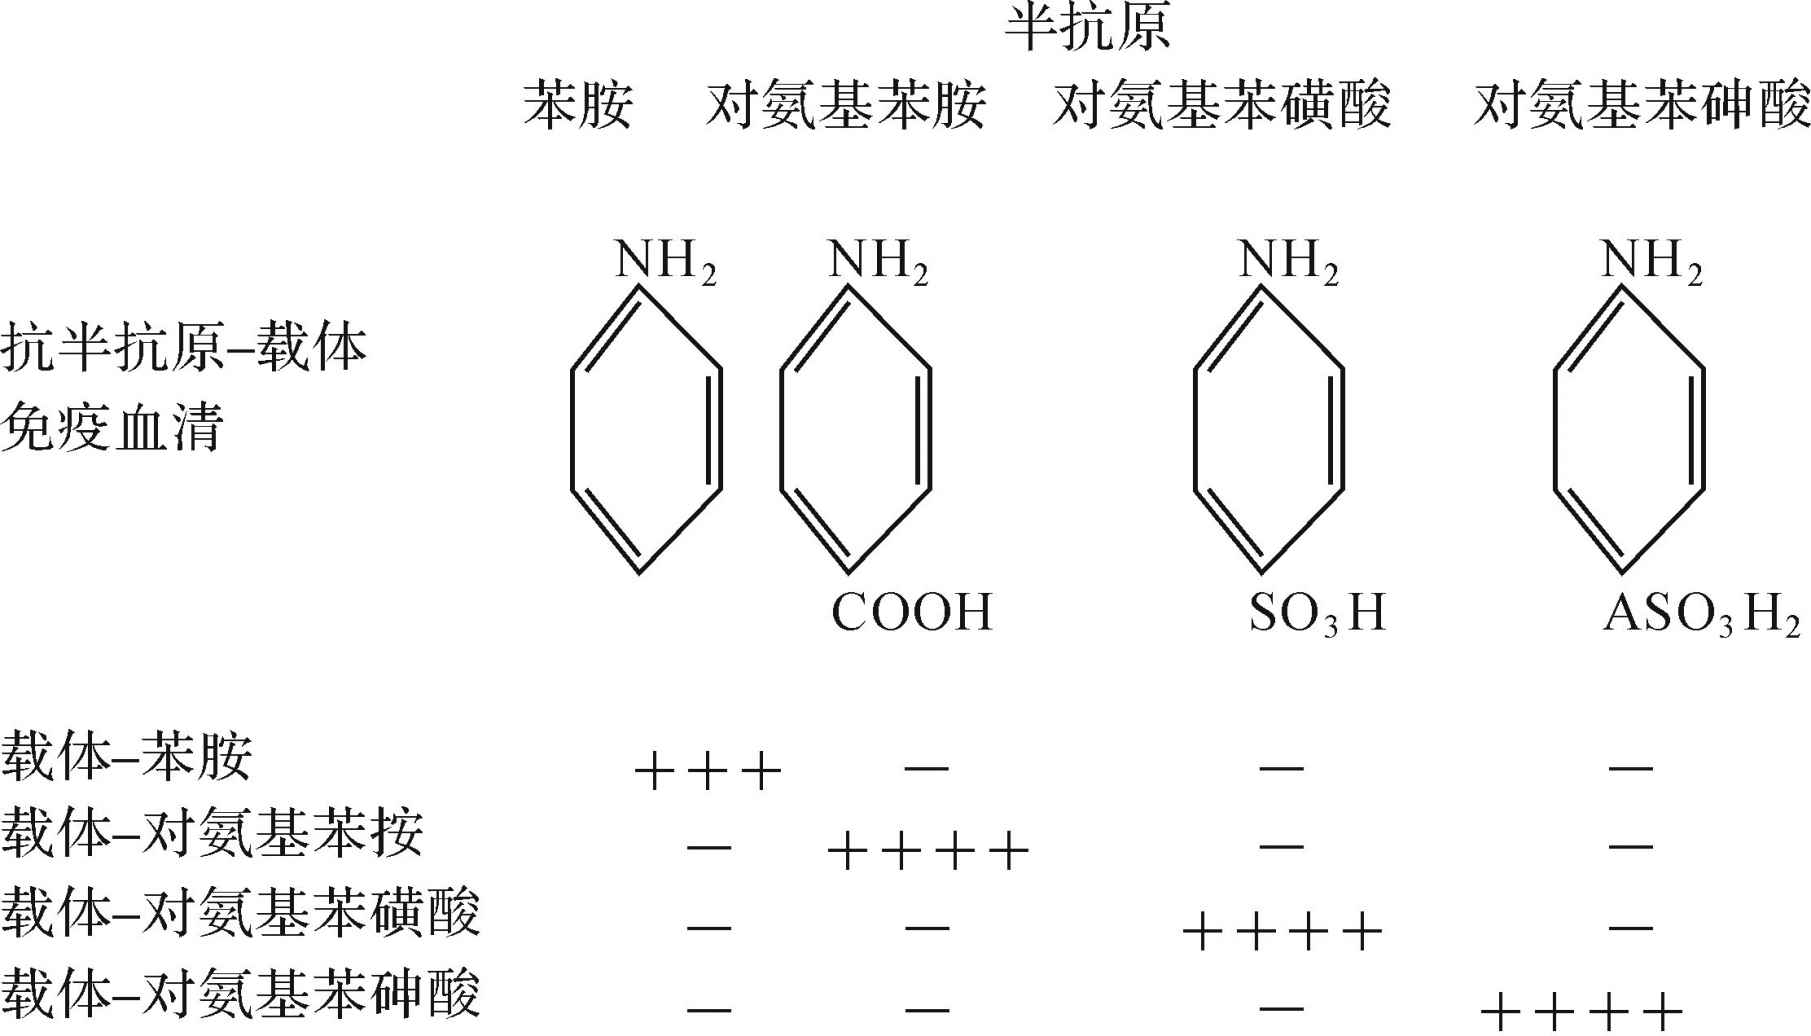
\includegraphics[width=.6\textwidth]{./images/Image00052.jpg}
 \captionsetup{justification=centering}
 \caption{抗原决定簇的性质决定抗原特异性}
 \label{fig3-3}
  \end{figure}

此外,多糖残基乃至单糖的微细差别也可导致抗原性的不同。例如:A型血和B型血红细胞表面抗原的区别仅在于前者是N-乙酰氨基半乳糖,而后者为L-岩藻糖。

5.顺序决定簇和构象决定簇:

依表位的结构特点可将表位分为两类:

(1)顺序表位(即连续性表位):主要由一段序列相连的氨基酸片段形成,多在抗原分子内。

(2)构象性表位(即非连续性表位):短肽、多糖残基或核苷酸并非简单的线性排列,而是形成特定的空间构象。

T细胞仅识别由抗原递呈细胞加工递呈的顺序表位,而B细胞可识别线性或构象性表位(图\ref{fig3-4})。

\begin{figure}[!htbp]
 \centering
 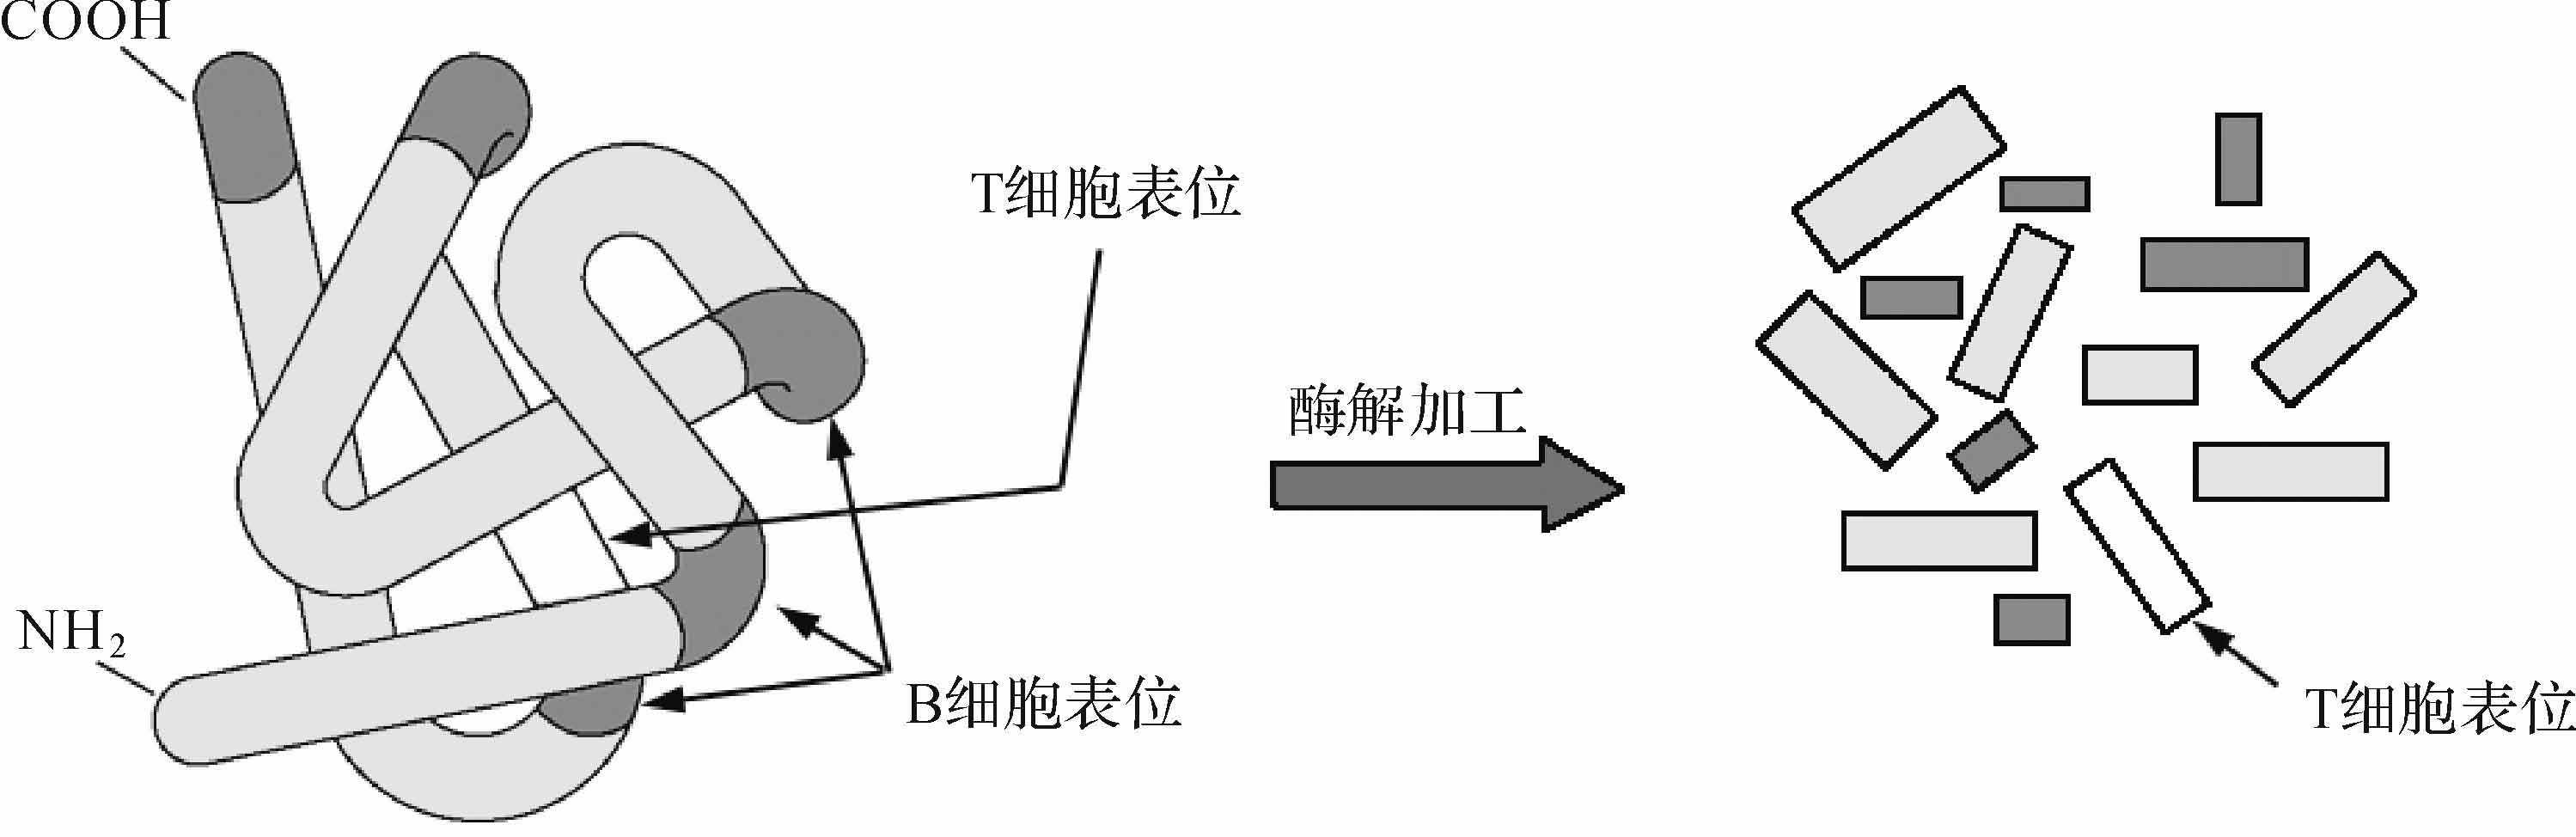
\includegraphics{./images/Image00053.jpg}
 \captionsetup{justification=centering}
 \caption{抗原的表位示意图}
 \label{fig3-4}
  \end{figure}

6.交叉反应和共有决定簇:

免疫系统可识别不同表位间的细微区别,从而显示免疫应答的特异性。但在实践中已发现,某些特定抗原不仅可与其诱导产生的抗体/致敏淋巴细胞结合或相互作用,还可与其他抗原诱生的抗体/致敏淋巴细胞发生反应被称为交叉反应(cross
reaction)(图\ref{fig3-5})。交叉抗原的存在和交叉反应现象的发生并非否定抗原的特异性,而是由于复杂抗原具有多个抗原决定簇,不同抗原之间存在相同或相似的抗原决定簇。如:流产布氏杆菌与肠耶尔森氏菌有交叉反应。

\begin{figure}[!htbp]
 \centering
 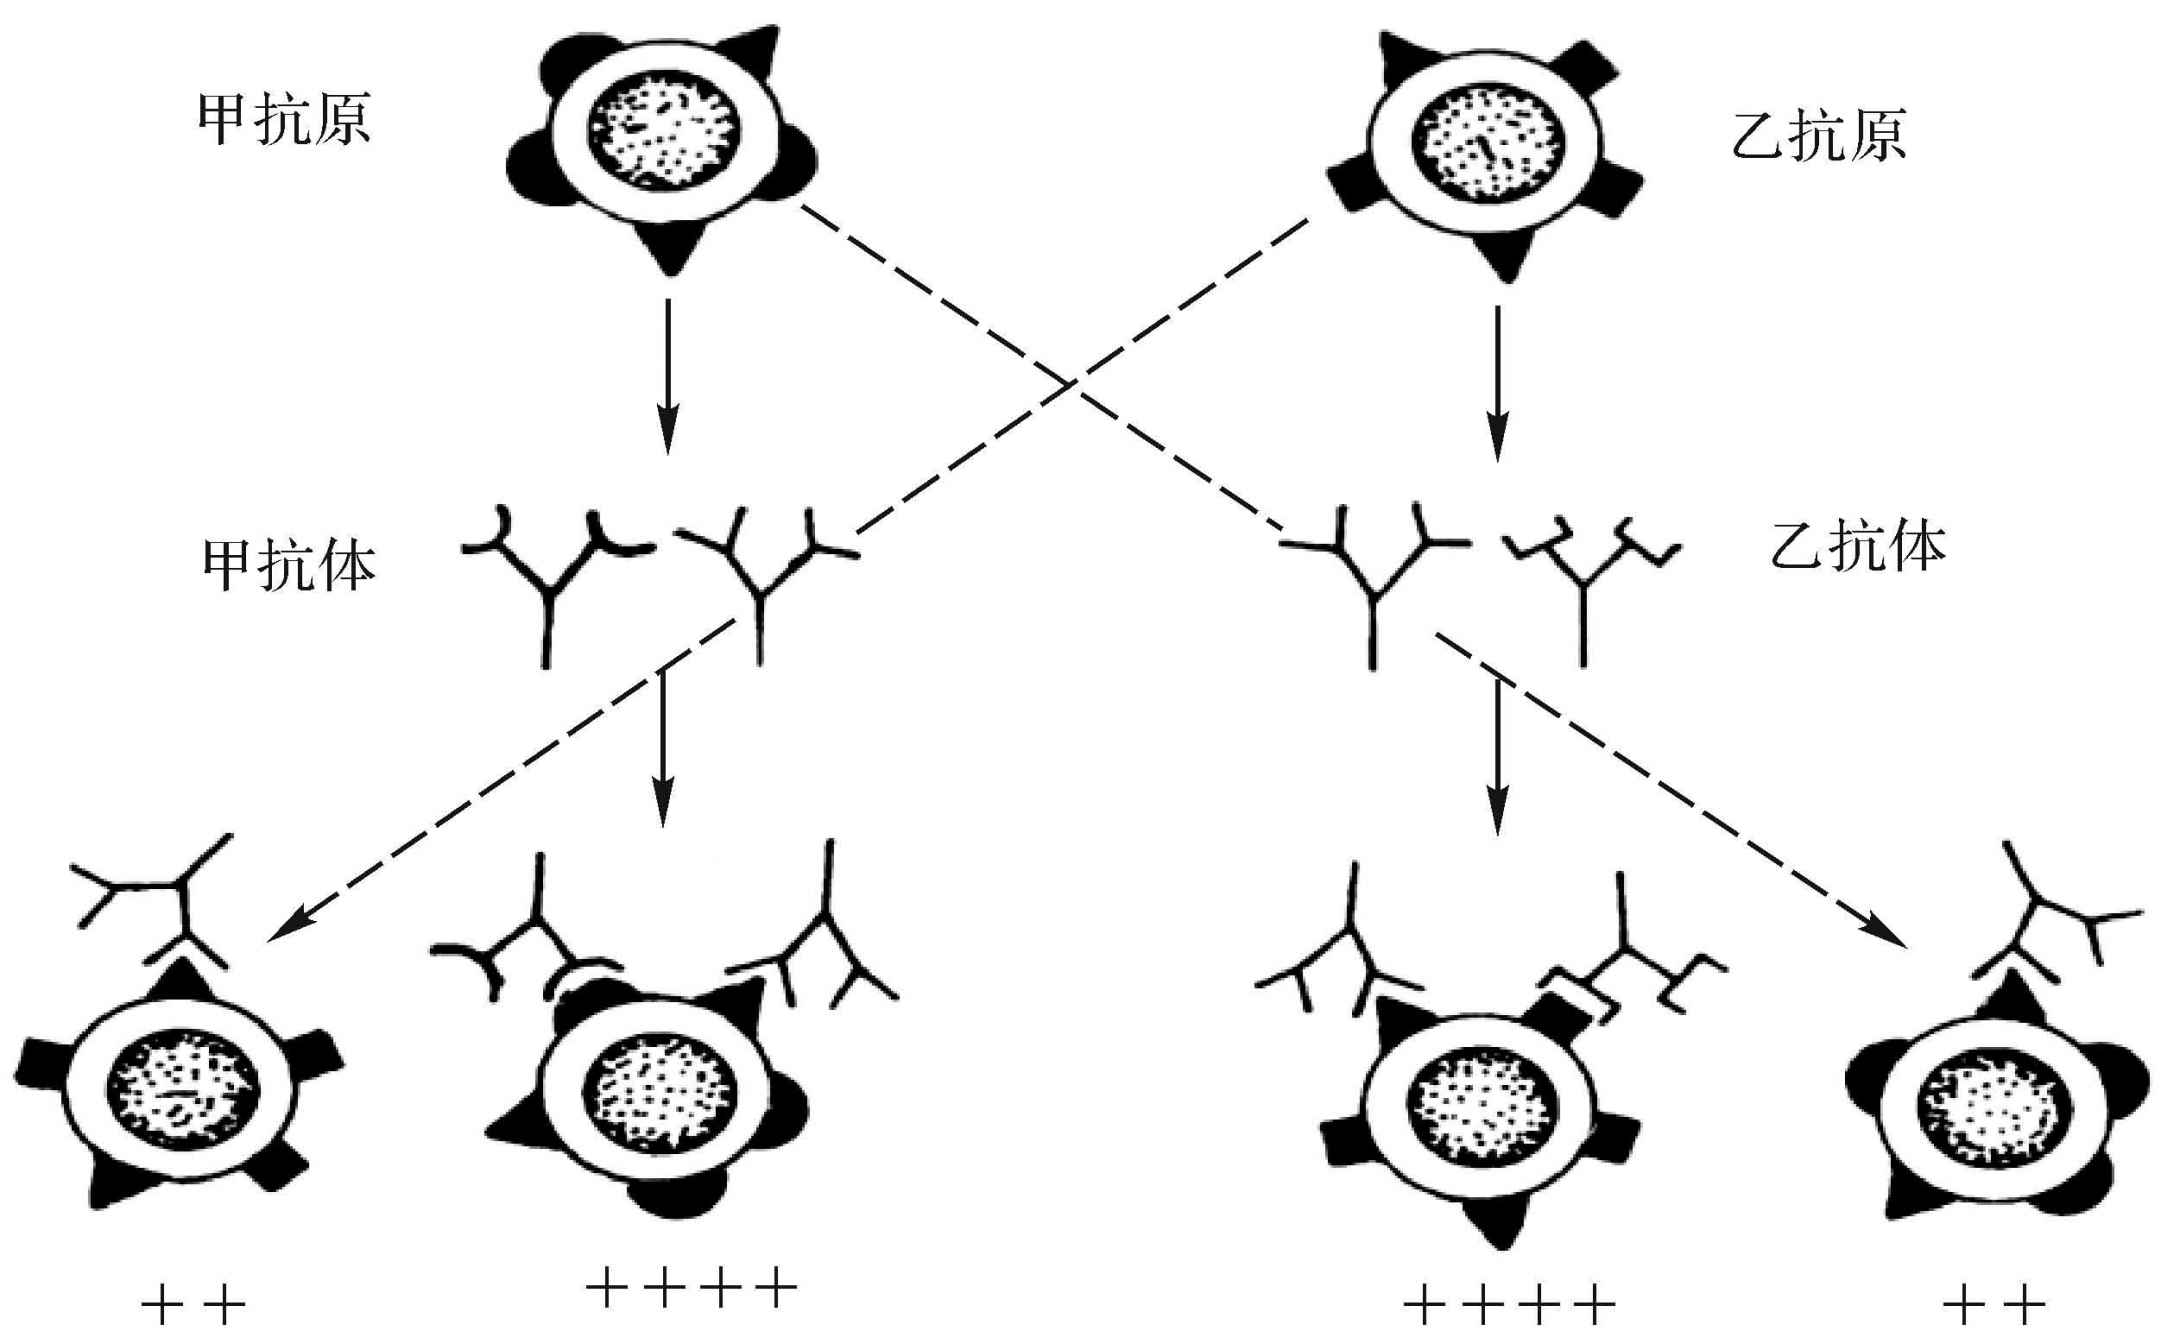
\includegraphics{./images/Image00054.jpg}
 \captionsetup{justification=centering}
 \caption{交叉反应}
 \label{fig3-5}
  \end{figure}

不同种属(如人、动物和微生物)间可存在共有决定簇,其生物学意义在于:

(1)某些情况下,针对病原微生物的免疫应答可导致对人体的免疫损伤。

(2)在进行特异性诊断或鉴定时,须排除交叉抗原可能产生的干扰。

(3)应用交叉抗原可能诱导出针对难于制备的抗原的免疫应答。例如近年报道,斑疹伤寒立克次氏体可诱导机体产生针对HIV的免疫应答。

\section{抗原的分类及其医学意义}


\subsection{依据抗原诱生抗体时对T细胞的依赖性}

依据抗原诱生抗体时对T细胞的依赖性将抗原分为胸腺依赖性抗原和非胸腺依赖性抗原(图\ref{fig3-6})。

1.胸腺依赖性抗原(thymus dependent antigen,TD
antigen):TD抗原亦称T细胞依赖抗原,其刺激机体产生抗体依赖于T细胞辅助,绝大多数蛋白质抗原及细胞抗原属TD抗原。先天性胸腺缺陷和后天性T细胞功能缺陷的个体,TD抗原诱导其产生抗体的能力明显低下。

2.非胸腺依赖抗原(thymus independent antigen,TI
antigen):TI抗原亦称T细胞非依赖性抗原,其刺激机体产生抗体无需T细胞辅助。TI抗原可分为两类:①TI-1抗原具多克隆B细胞激活作用,如细菌脂多糖(LPS)即为典型的TI-1抗原,成熟或未成熟B细胞均可对其产生应答;②TI-2抗原表面含多个重复表位,如肺炎荚膜多糖、聚合鞭毛素等,它们只能刺激成熟B细胞。

\begin{figure}[!htbp]
 \centering
 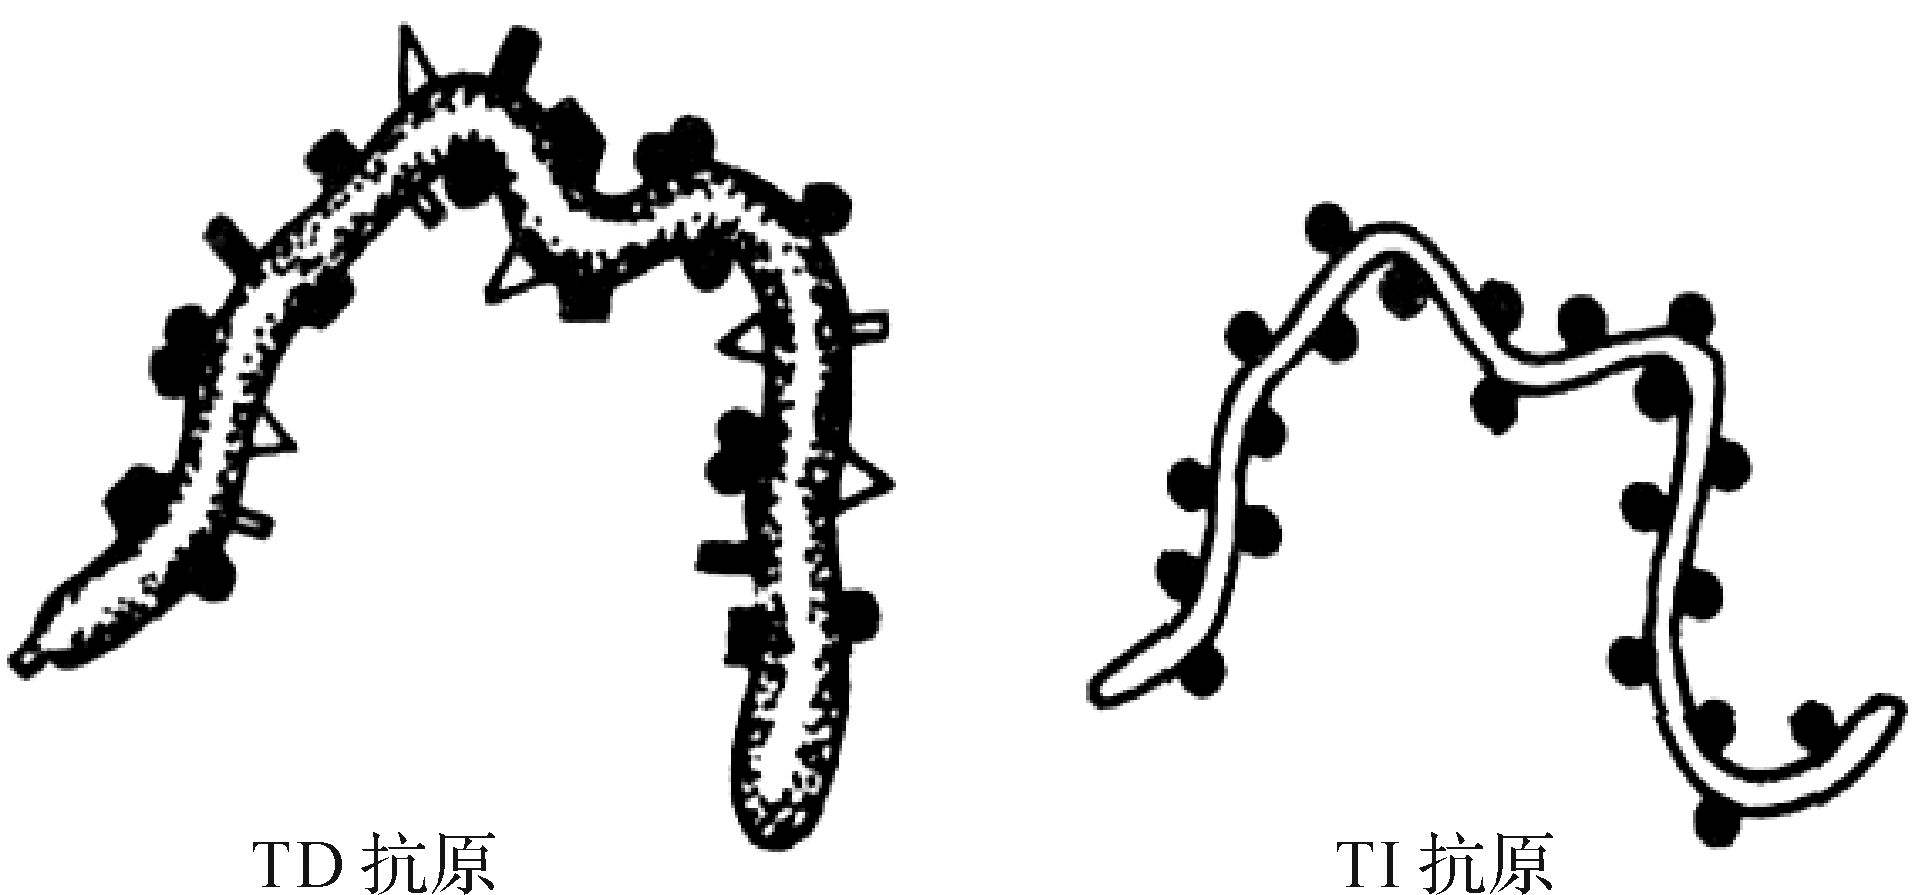
\includegraphics{./images/Image00055.jpg}
 \captionsetup{justification=centering}
 \caption{TD抗原与TI抗原结构示意图}
 \label{fig3-6}
  \end{figure}

\begin{figure}[!htbp]
 \centering
 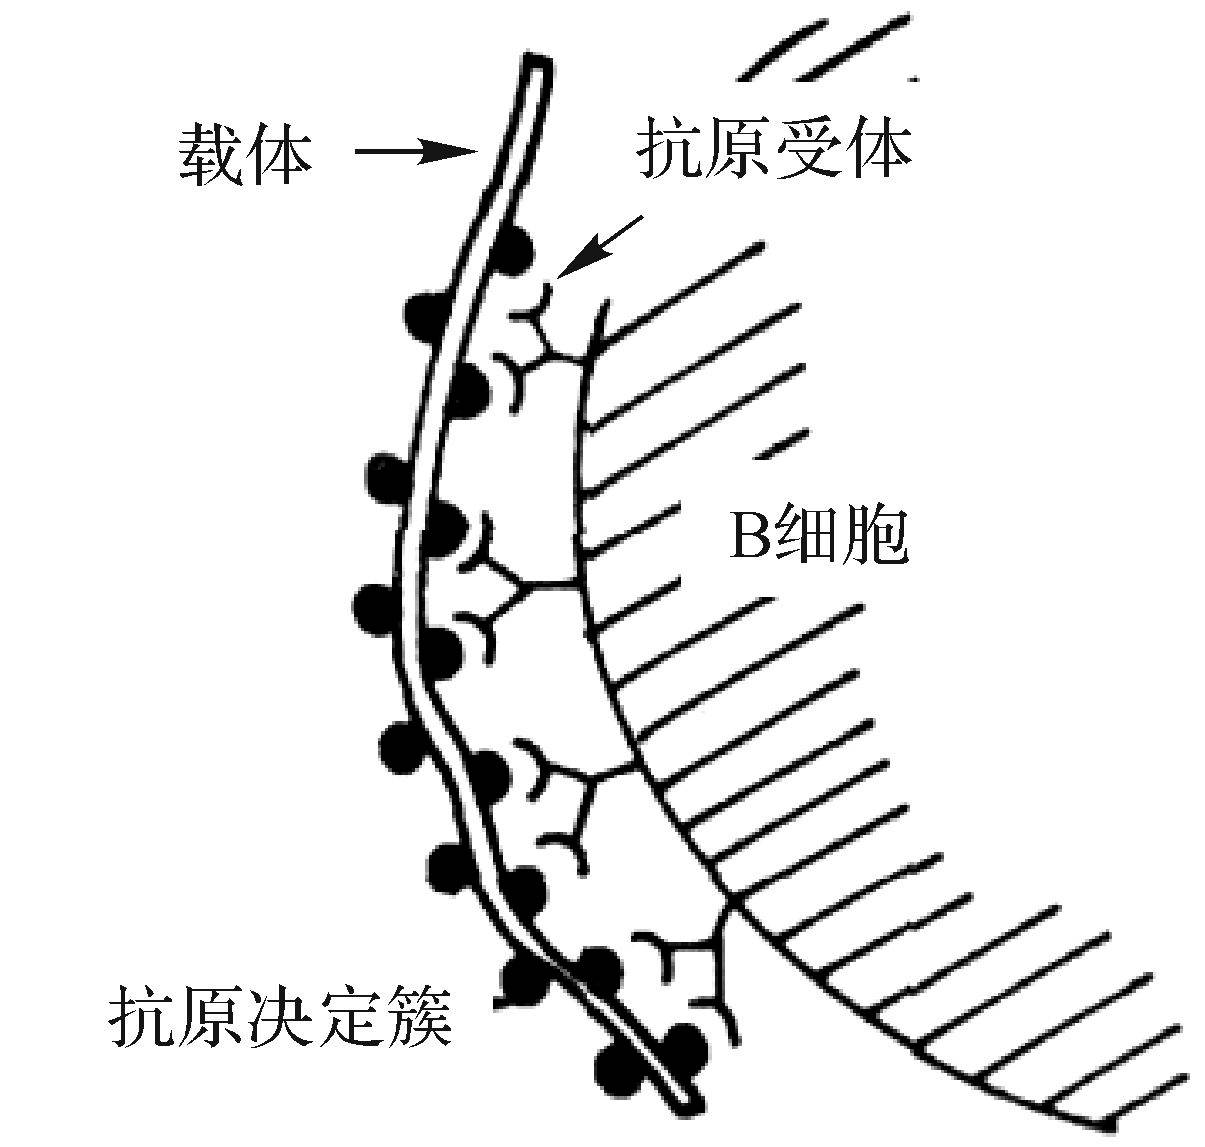
\includegraphics{./images/Image00056.jpg}
 \captionsetup{justification=centering}
 \caption{TI抗原激活B细胞示意图}
 \label{fig3-7}
  \end{figure}


\subsection{根据抗原与机体的亲缘关系}

1.异种抗原(xenogenic
antigen):指来自不同种属的抗原。对人类而言,病原微生物及其产物、植物蛋白、用于治疗目的的动物抗血清及异种器官移植物等均为重要的异种抗原。

2.同种异型抗原(allogenic
antigen):亦称同种抗原(或人类的同种异体抗原),指同一种属不同个体所具有的特异性抗原。重要的人类同种异型抗原包括:①红细胞血型抗原,包括ABO、Rh等40余个抗原系统,其对安全输血极为重要;②人类主要组织相容性抗原,即人白细胞抗原(HLA),是具有高度多态性的抗原系统。另外,同一种属不同个体的同类免疫球蛋白也存在抗原性的差异,即免疫球蛋白的同种异型(allotype)。

3.自身抗原(autoantigen):正常情况下,机体免疫系统不对自身正常组织或细胞产生免疫应答,即处于自身耐受状态。在某些病理情况下(如隐蔽抗原或隔离抗原释放;自身抗原发生改变或被修饰等),自身抗原成分可诱导机体产生自身免疫应答。

4.异嗜性抗原(heterophilic
antigen):是一类与种属无关,存在于人、动物及微生物之间的共同抗原,又称Forssman抗原。例如,A族溶血性链球菌表面成分与人肾小球基底膜及心肌自身组织具有共同抗原,故溶血性链球菌感染后,其刺激机体产生的抗体可能与具有共同抗原的心、肾组织发生交叉反应,导致肾小球肾炎或心肌炎。


\subsection{根据(TD)抗原是否由抗原递呈细胞所合成}

1.外源性抗原(exogenous
antigen):来源于抗原递呈细胞之外、不由其合成的抗原称为外源性抗原,如被抗原递呈细胞吞噬的细胞或细菌等。此类抗原由抗原递呈细胞摄取、加工为抗原肽,进而与MHC-Ⅱ类分子结合为复合物,由CD\textsuperscript{+}
\textsubscript{4} T细胞的TCR识别。

2.内源性抗原(endogenous
antigen):由抗原递呈细胞在其胞内合成的抗原称为内源性抗原(如病毒感染细胞合成的病毒蛋白、肿瘤细胞内合成的肿瘤抗原等)。此类抗原被加工为抗原肽并与MHC-Ⅰ类分子结合成复合物,由CD\textsuperscript{+}
\textsubscript{8} T细胞的TCR识别。

\begin{figure}[!htbp]
 \centering
 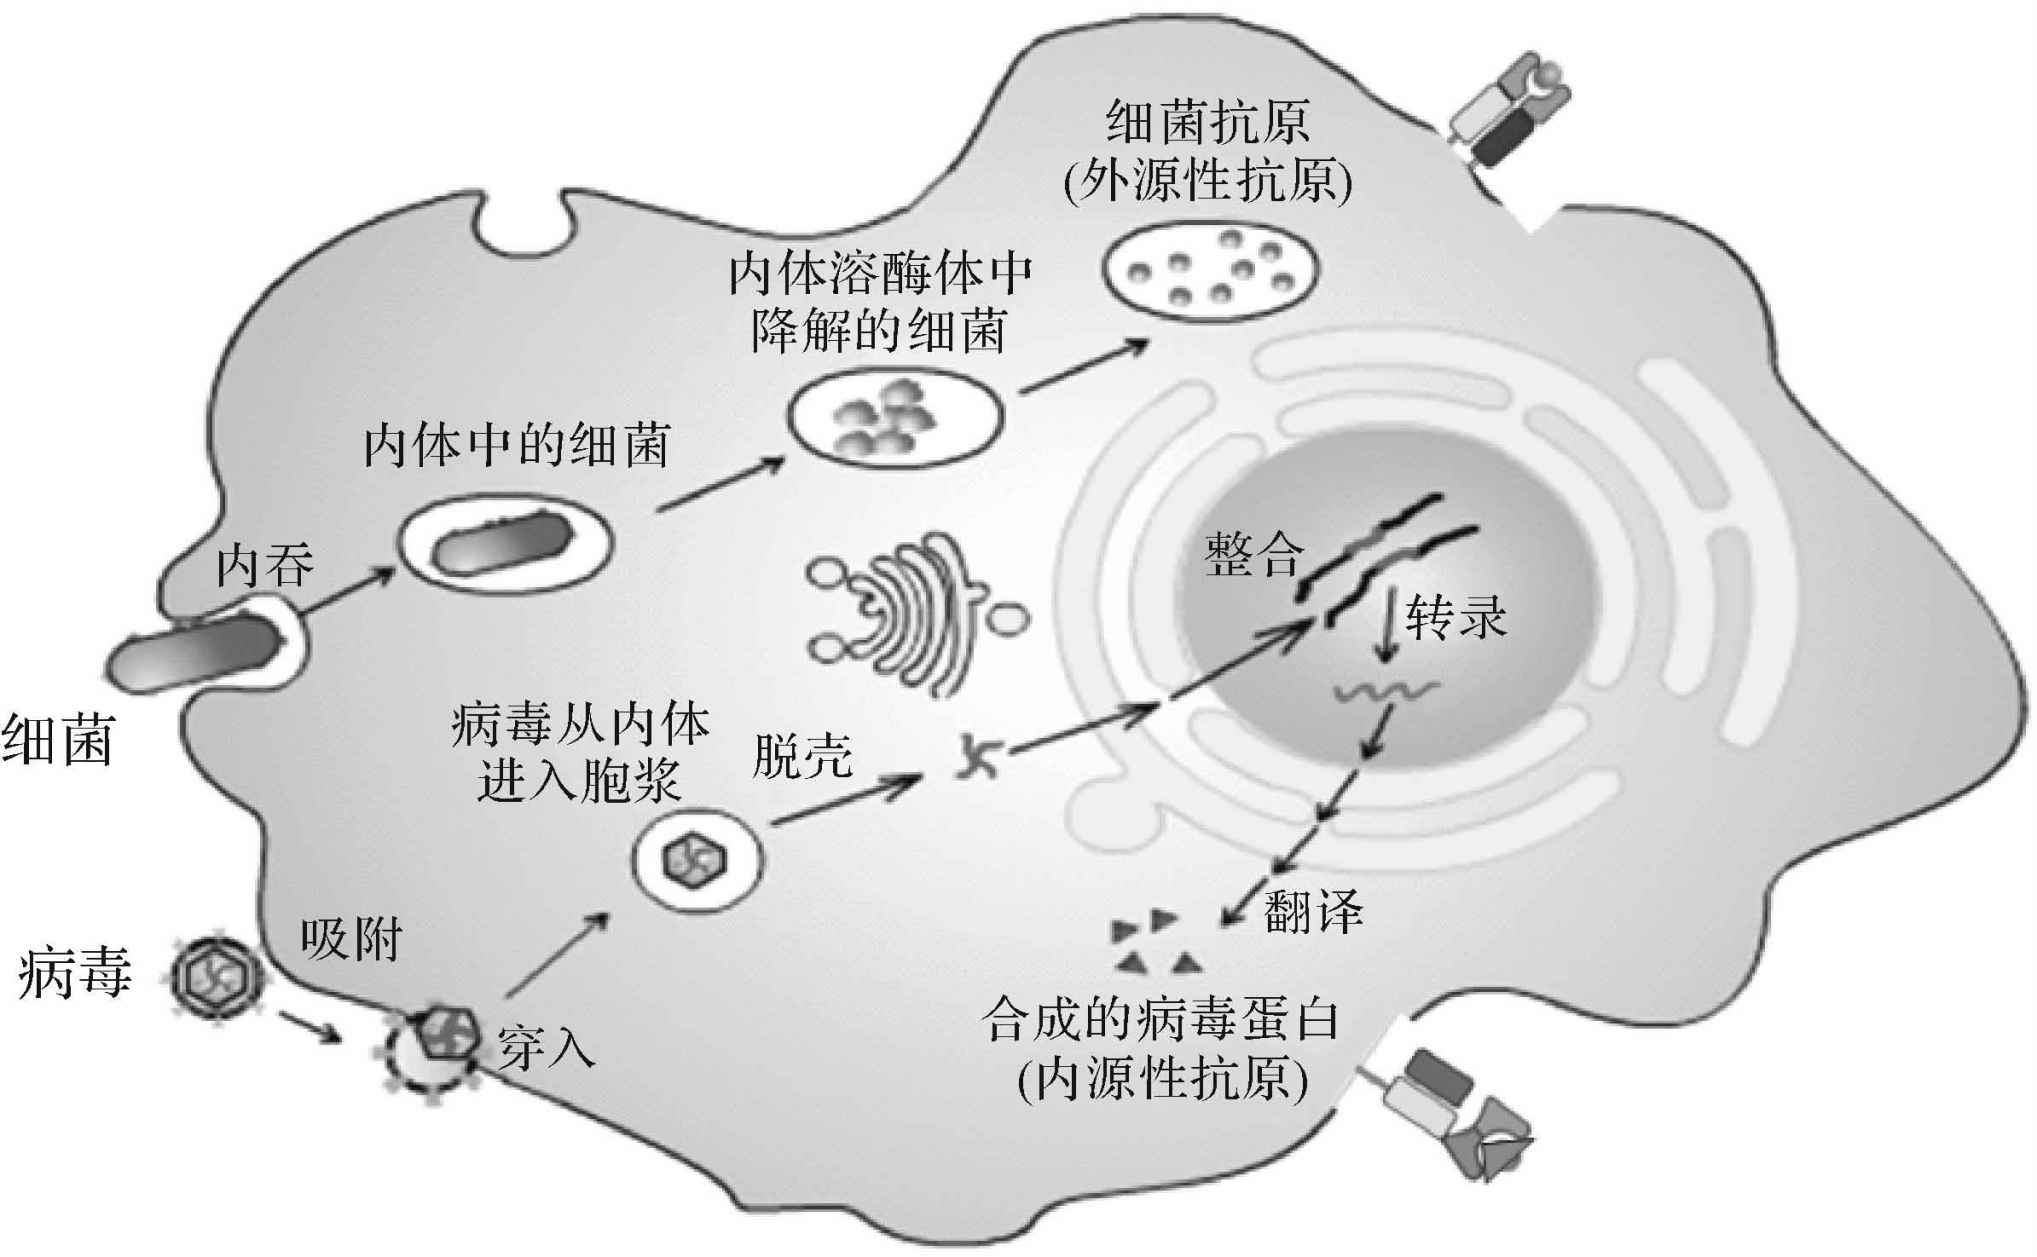
\includegraphics{./images/Image00057.jpg}
 \captionsetup{justification=centering}
 \caption{外源性抗原与内源性抗原}
 \label{fig3-8}
  \end{figure}


\subsection{根据来源}

(一)细菌的抗原

(1)表面抗原:细胞壁外的抗原物质,如K抗原(大肠杆菌)、Vi抗原(伤寒杆菌)。

(2)菌体抗原:细胞壁中的抗原物质:O抗原。

(3)鞭毛抗原:鞭毛中的抗原物质:H抗原。

(4)菌毛抗原。

细菌结构如图\ref{fig3-9}所示。

\begin{figure}[!htbp]
 \centering
 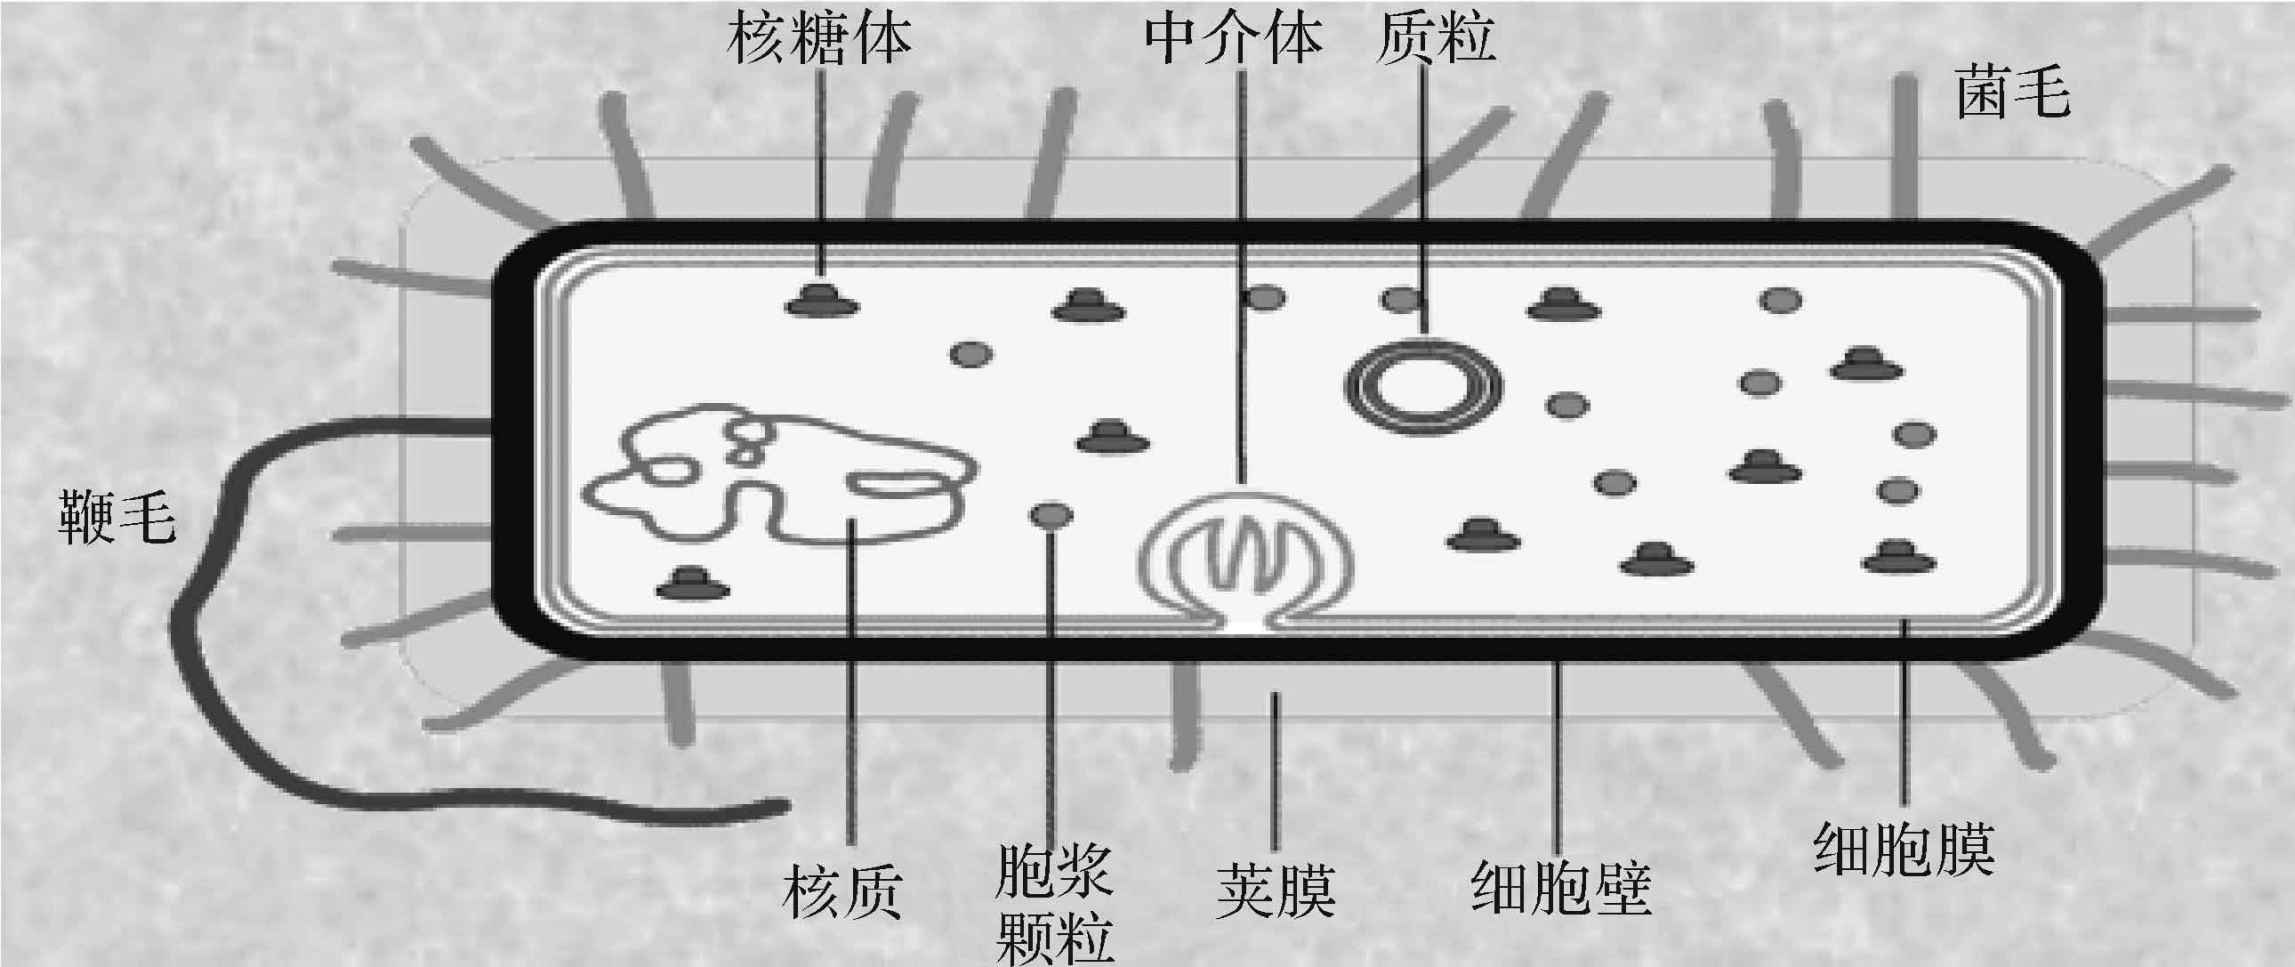
\includegraphics{./images/Image00058.jpg}
 \captionsetup{justification=centering}
 \caption{细菌结构示意图}
 \label{fig3-9}
  \end{figure}

(5)类毒素:经0.3\%~0.4\%甲醛处理过的失去毒性保留免疫原性的外毒素。如:白喉类毒素、破伤风类毒素。

(二)肿瘤抗原

肿瘤抗原是指细胞癌变过程中出现的新抗原及过度表达的抗原物质的总称。

1.肿瘤特异性抗原(tumor specific antigen
TSA):肿瘤细胞特有的或只存在于某种肿瘤细胞而不存在于正常细胞的新抗原。

如:前列腺特异性抗原(PSA):正常情况下小于4.0μg/L。

2.肿瘤相关抗原(tumor associated antigen
TAA):非肿瘤细胞所特有的、正常细胞和组织也存在的抗原,只是其含量在细胞癌变时明显增加。

如:甲胎蛋白(AFP):正常成人血清中的AFP小于20μg/L;肝癌患者的AFP大于500μg/L。癌胚抗原(CEA):正常血清中的CEA小于2-5μg/L。


\subsection{其他分类}

根据抗原的理化性质,可分为颗粒抗原(细菌性、细胞性等)、可溶性抗原(牛血清白蛋白、菌脂多糖等)、蛋白抗原、多糖抗原及多肽抗原等。

\section{非特异性免疫刺激剂}

除了抗原可以诱导特异性免疫应答,还存在非特异性激活B细胞、T细胞的物质。


\subsection{免疫佐剂}

免疫佐剂是指那些与抗原一起或先于抗原注入机体后可增强抗原的免疫原性,即辅佐抗原的作用。此类物质被称为佐剂(adjuvant)。本质上,佐剂可视为一种非特异性免疫增强剂,可增强体液免疫与细胞免疫应答。

(一)佐剂的种类

1.化合物:包括氢氧化铝、明矾、矿物油及吐温80、弗氏不完全佐剂(羊毛脂与石蜡油的混合物),以及人工合成的多聚肌苷酸,如胞苷酸(Poly
I:C)、脂质体等。

2.生物制剂:①经处理或改造的细菌及其代谢产物,如卡介苗、短小棒状杆菌、百日咳杆菌,以及霍乱毒素B亚单位(CTB)、革兰阴性菌细胞壁成分脂多糖(LPS)和类脂A、源于分支杆菌的胞壁酰二肽等;②细胞因子及热休克蛋白等。

迄今能安全用于人体的佐剂仅限于氢氧化铝、明矾、PolyI:C、胞壁酰二肽、细胞因子及热休克蛋白等。最常用于动物实验的佐剂是弗氏完全佐剂(弗氏不完全佐剂加卡介苗)和弗氏不完全佐剂。

(二)佐剂的作用机制

1.改变抗原的物理性状,延缓抗原降解和排除,从而更有效地刺激免疫系统;

2.刺激单核/巨噬细胞系统,增强其处理和递呈抗原的能力;

3.刺激淋巴细胞增殖与分化。

(三)佐剂的应用

1.增强特异性免疫应答,用于预防接种及制备动物抗血清;

2.作为非特异性免疫增强剂,用于抗肿瘤与抗感染的辅助治疗。


\subsection{超抗原}

由White于1989年提出,是一类由细菌外毒素和逆转录病毒蛋白构成的抗原性物质,只需极低浓度(1-10μg/L)即能激活T细胞产生很强的免疫应答。迄今已发现的超抗原包括金黄色葡萄球菌肠毒素A~E(SEA~E)、表皮剥脱毒素(EXT)、关节炎支原体丝裂原(MAM)、小肠结肠耶氏菌膜蛋白及小鼠逆转录病毒的蛋白产物等。

1.超抗原的作用特点

超抗原的作用特点如图\ref{fig3-10}所示。

\begin{figure}[!htbp]
 \centering
 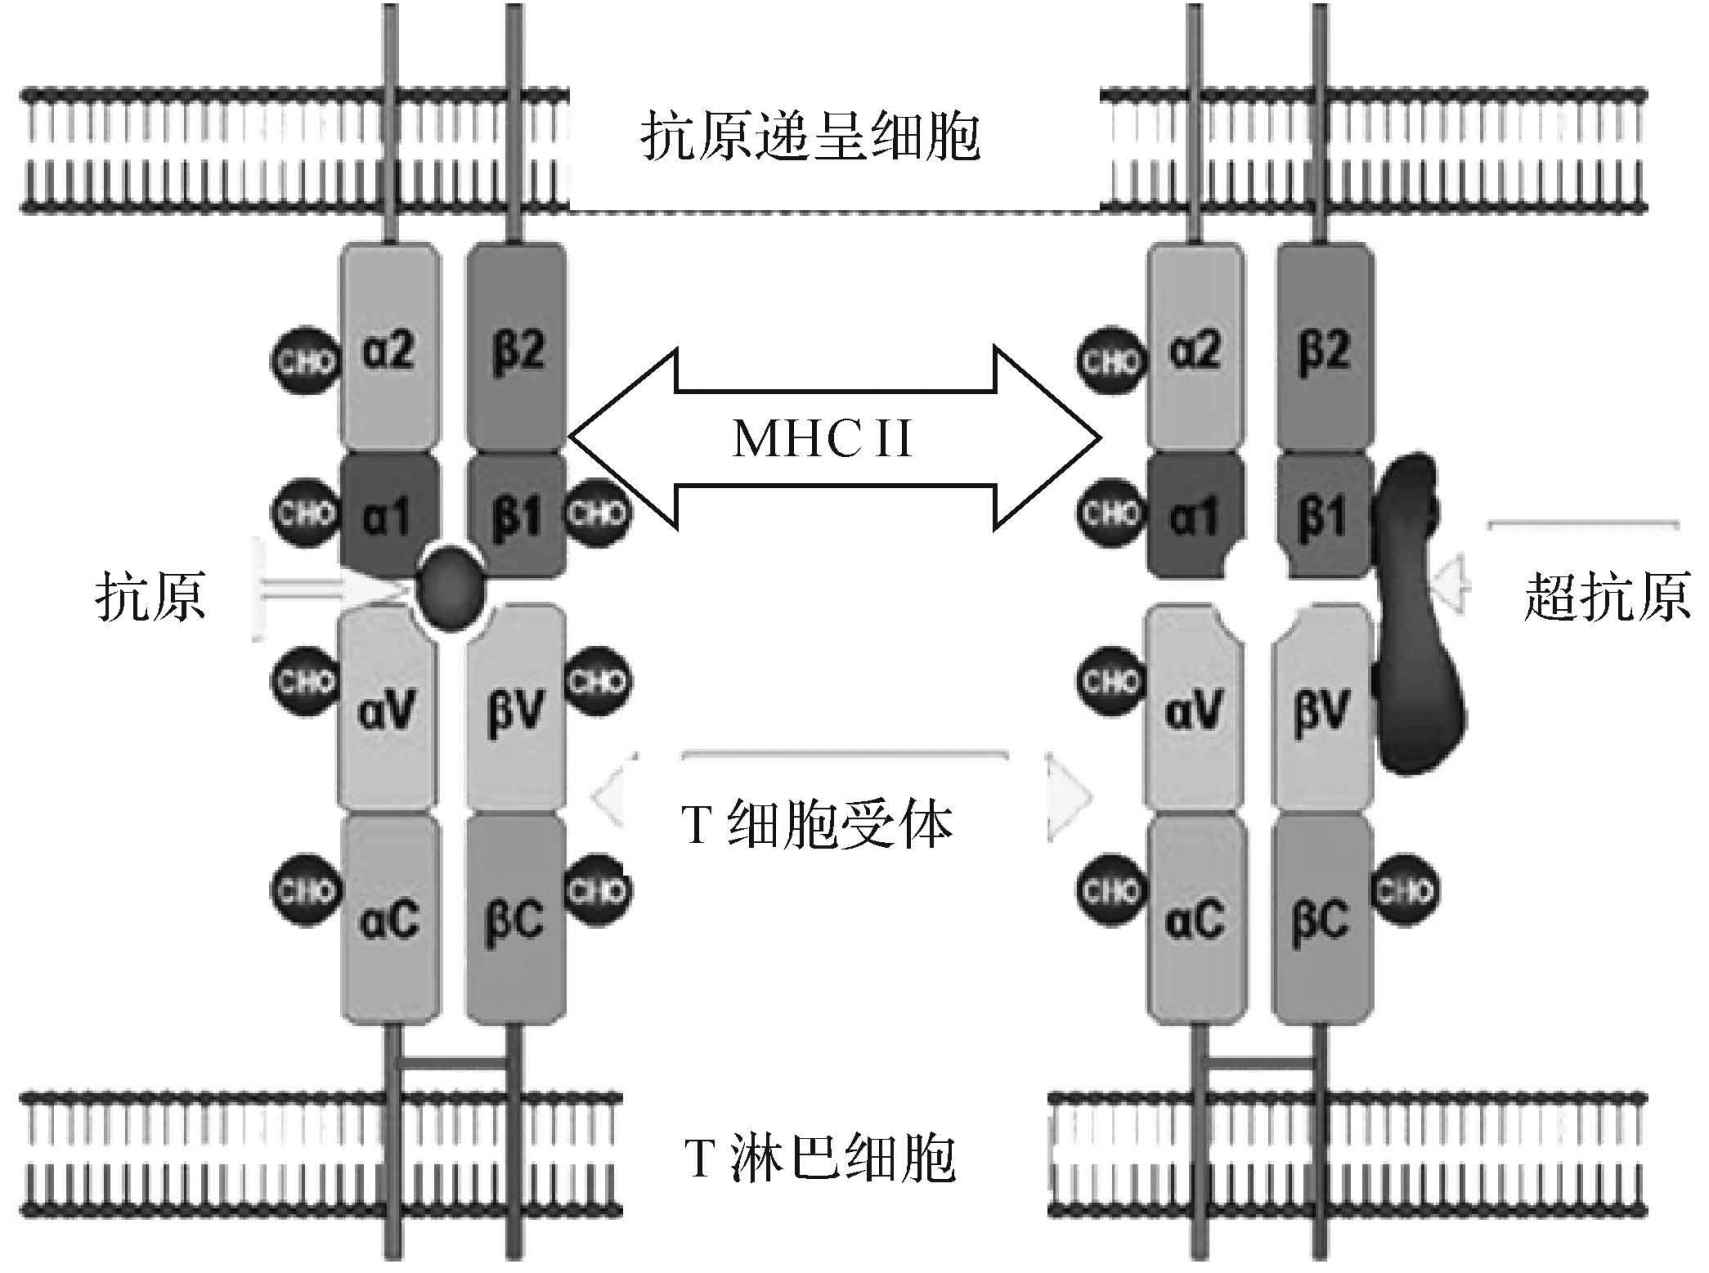
\includegraphics[width=.6\textwidth]{./images/Image00059.jpg}
 \captionsetup{justification=centering}
 \caption{超抗原作用示意图}
 \label{fig3-10}
  \end{figure}

(1)无须抗原加工与递呈,可直接与MHC-Ⅱ类分子结合。

(2)形成TCR
Vβ-超抗原-MHC-Ⅱ类分子复合物,而非普通抗原的TCR-抗原肽-MHC-Ⅱ类分子复合物。

(3)尽管超抗原发挥作用有赖于与MHC分子结合,但其作用无MHC限制性。

(4)所诱导的T细胞应答,其效应并非针对超抗原自身,而是通过分泌大量细胞因子而参与某些病理生理过程的发生与发展。依据上述功能特点,超抗原也被视为一类多克隆激活剂。此外,近年还发现了作用于B细胞的超抗原。

2.超抗原的生物学意义在于:

(1)毒性作用及诱导炎症反应:由于超抗原多为病原微生物代谢产物,可大量激活T细胞并诱导炎性细胞与促炎细胞因子产生,从而引起休克等严重反应(如食物中毒时金葡菌肠毒素所致休克等严重临床表现)。

(2)自身免疫病:超抗原可通过激活体内残存的自身反应性T细胞而导致自身免疫病。

(3)免疫抑制:受超抗原刺激而过度增殖的大量T细胞,可被清除或功能上出现超限抑制,从而导致微生物感染后的免疫抑制。

3.超抗原与普通抗原的比较

超抗原与普通抗原的比较归纳如表\ref{tab3-1}。

\begin{longtable}[]{@{}lll@{}}
    \caption{超抗原与普通抗原的比较}
    \label{tab3-1}\\
\toprule
特 点 & 普通抗原 & 超抗原\tabularnewline
\midrule
\endhead
物质属性 & 蛋白质、多糖 & 细菌外毒素、逆转录病毒蛋白\tabularnewline
应答特点 & 由 APC处理后被 T细胞识别 & 直接刺激 T细胞\tabularnewline
反应细胞 & T细胞、B细胞 & CD\textsuperscript{+} \textsubscript{4}
T细胞\tabularnewline
T细胞反应频率 & 1/10\textsuperscript{6} -10\textsuperscript{4} &
120-15\tabularnewline
与 MHC分子结合部分 & 多态区肽结合槽 & 非多态区\tabularnewline
MHC限制性 & + & -\tabularnewline
\bottomrule
\end{longtable}


\subsection{丝裂原}

丝裂原(mitogen)亦称有丝分裂原,可致细胞发生有丝分裂,进而增殖。体外实验中,特定丝裂原可使静止的淋巴细胞体积增大、胞浆增多、DNA合成增加,出现淋巴母细胞化即淋巴细胞转化(lymphocyte
transformation)和有丝分裂。

如前所述,一种特定的抗原仅特异性激活表达相应抗原受体的淋巴细胞,而丝裂原可激活某一类淋巴细胞的全部克隆,故可将丝裂原视为非特异性多克隆激活剂。T、B淋巴细胞表面表达多种丝裂原受体,故均可对丝裂原刺激产生增殖反应,这一性质已被用于在体外检测淋巴细胞的应答能力(如淋巴细胞转化试验),并以此评价机体的免疫功能。表\ref{tab3-2}所列出的是作用于人和小鼠T、B细胞的重要丝裂原。
 
\begin{longtable}[]{lllll}
    \caption{作用于人和小鼠T、B细胞的重要丝裂原}
    \label{tab3-2}\\
\toprule
丝裂原 & \multicolumn{4}{c}{对 T、B细胞的促增殖作用} \\
&人T细胞&人B细胞&小鼠T细胞&小鼠B细胞\\
\midrule
\endhead
刀豆蛋白 A&+&-&+&-\\
植物血凝素&+&-&+&-\\
脂多糖&-&-&-&+\\
葡萄球菌A蛋白&-&+&-&-\\
\bottomrule
\end{longtable}



\noindent\textbf{【理解与思考】}

1.什么样的人与事对你印象特别深?满足哪些条件的物质对机体的免疫原性强?

2.你能形象地描绘抗原的特异性与抗原决定簇、抗原表位性质与位置的关系吗?

3.结合生产与生活实际,描述共有决定簇与特异性抗原决定簇的应用。

4.你能将免疫佐剂的作用形象描绘一下吗?

5.你能辩证说明抗原与免疫细胞的关系吗?

\noindent\textbf{【课外拓展】}

1.抗原在临床实践中有什么应用?

2.自身抗原会导致机体处于什么状态?

3.癌变细胞为什么会表达肿瘤抗原?

4.超抗原在医学上有何意义?

\noindent\textbf{【课程实验与研究】}

1.从抗原的角度出发,请设计一种方案来增强机体的免疫力。

2.选择某种免疫佐剂,研究其在体内的作用机理。

3.如何去鉴定某种抗原物质具有多少抗原决定簇?

4.如何检测某种物质是否是超抗原?

5.请设计一方案,研究异嗜性抗原对机体的影响。

6.Sci Transl
Med在2010年1月20日报道称“佐剂可大大增强流感疫苗功效”。请你设计一方案,证明其功效。

\noindent\textbf{【课程研讨】}

1.基因工程疫苗与传统的疫苗相比有何区别?如何增强基因工程类疫苗的免疫原性?

2.细菌中有哪些成分可以成为抗原物质?在细菌分类与鉴别上有什么意义?

3.细菌性抗原、病毒性抗原有什么不同?引起机体免疫应答有何差异?

4.不同的免疫佐剂在医学上各有何应用?请比较其不同特点。

5.超抗原在目前的应用进展如何?

\noindent\textbf{【课后思考】}

1.什么是抗原? 其特性是什么?

2.决定免疫原性的因素有哪些?

3.抗原的特异性与抗原决定簇有何关系?

4.名词解释:异嗜性抗原;TD-Ag;TI-Ag;超抗原;免疫佐剂。

\noindent\textbf{【课外阅读】}

\begin{center}
    \textbf{\Large 超抗原及其应用前景}
\end{center}

早在20世纪70年代,金黄色葡萄球菌能大量激活外周血细胞而造成休克、发热、脱水、皮疹及多器官衰竭的毒素休克征的现象已被人们熟知。但直至
1989 年,White
博士才首次提了超抗原(Superantigen,SAg)的概念。超抗原是一类特殊的抗原,是功能非常活跃的蛋白质分子,主要由一些细菌、病毒、支原体及寄生虫等微生物的分泌物或代谢产物组成。与普通抗原相比,它不需要抗原递呈细胞加工处理可直接与
MHC类分子结合形成配体,然后该配体进一步与 TCR
VB区结合形成三聚体激活多克隆T细胞,具极高的T细胞激活频率。超抗原具有独特的特点:
①强大的刺激能力;②无须抗原递呈细胞的处理;③无
MHC的限制;④广泛的T细胞识别特性;⑤选择性结合T细胞受体(T cell
recepter,TCR)β链V区。

\begin{center}
{\large 一、SAg作用的分子机制}
\end{center}

超抗原分子按其作用的细胞种类,可分为T细胞超抗原及
B细胞超抗原。T细胞超抗原即我们通常意义上的超抗原概念,B细胞超抗原则为一类新型超抗原分子,与T细胞超抗原特性一致,但作用方式不尽相同,它能刺激B细胞产生大量免疫球蛋白,激活体液免疫反应和补体级联反应。

(一)T细胞超抗原

T细胞超抗原能非特异激活大量
T细胞,它不遵循传统的抗原递呈途径,不经抗原递呈细胞胞内加工处理而是以完整的蛋白质分子直接结合到MHC类分子上。结合部位不在抗原肽结合的沟槽内,而在沟槽外侧。SAg与
MHC 分子的相互作用对于激活 T细胞是很重要的。SAg通过与 MHC类分子和 TCR
形成一个三元复合物来激活
T细胞,对T细胞的激活频率在5\%~30\%左右,比普通抗原高10\textsuperscript{3}
~10\textsuperscript{5}
倍。所以极微量超抗原(pMol)就能诱导机体产生免疫应答。SAg的另一特点是能同等激活
CD4\textsuperscript{+} 和 CD8\textsuperscript{+} 两个亚群的 T
细胞,而普通抗原仅激活CD4\textsuperscript{+}
T细胞。近年来对超抗原结构和功能关系的研究很多,以葡萄球菌肠毒素为例,通过分析毒素多肽片段、毒素缺失和点突变体的活性,已测定出肠毒素激活T细胞的功能区域。
在此基础上,通过X射线晶体衍射测定出肠毒素分子、肠毒素与 MHC
类分子(HLD-DR)以及 TCR复合物的三维结构。

(二)B细胞超抗原

B细胞超抗原能刺激
B细胞产生大量免疫球蛋白,激活体液免疫和补体级联反应。目前认为
B细胞超抗原对VH基因家族成员的特异性与 T2SAg对
TCRVB的特异性相类似,它具有与血清中及
B细胞上相应受体(Ig)相互作用的能力,其中最具代表性的是
42KD的金黄色葡萄球菌蛋白SpA。不到0.01\%的B细胞能接受普通抗原特异性刺激,而SpA能结合约40\%的人多克隆IgM。正常细胞上有大量SpA受体,人外周B细胞约30\%能通过Ig-Fab介导结合SpA。

\begin{center}
    {\large 二、超抗原与疾病}
\end{center}

超抗原的生物学活性与其致病机制密切相关,激活T细胞分泌
TNF、IFN-γ、IL-2、IL-6、IL-10
等过量的细胞因子是引起中毒性休克症状的主要原因。微量的SAg就能诱导机体产生最大免疫应答,引起病情快、多器官损伤的系统性疾病。SAg与有些疾病的直接关系还没有证明,但诸如SAg在食物中毒、中毒性休克和自身免疫病中的作用已比较清楚。

(一)中毒性休克和食物中毒

SAg在人和鼠等许多动物内引起休克,体内注射 SAg导致 T细胞和
APC细胞激活,很快刺激产生 IL-2、TNF、IL-6 和
IFN-γ等细胞因子,导致体重下降和休克症状。对人多引起毛细血管渗漏,导致致死性休克。T细胞激活与超抗原介导的中毒性休克有关,已在动物和临床实验中得到证明。体外用TSST-1刺激人T细胞表现出VB2的优势表达,在中毒性休克病人的外周血中可检测到递呈VB2\textsuperscript{+}
T细胞。

(二)自身免疫性疾病

健康人的T、B外周血淋巴细胞不与自身抗原反应,但SAg可以激活自身反应性T细胞并介导T、B细胞相互作用引起自身免疫病。SAg激活的自身抗原特异性T细胞是引起自身免疫病的主要原因。通过单克隆抗体等方法封闭TCR
位点,部位消除和抑制这些
T细胞的作用可使病人的症状明显改善。SAg刺激产生的细胞因子引起非特异性损伤也与自身免疫疾病有关。另有说法认为,细菌SAg和热休克蛋白(HSP)有同源序列,而对HSP的免疫应答与自身免疫病的病理生理有关。类风湿关节炎患者血清中存在能产生自身抗体的B细胞,主要是CD5\textsuperscript{+}
B细胞亚群,类风湿因子是一种自身抗体,它能结合SpA和pFv,在关节炎患者关节液和循环体液中,VH3基因产物占85\%以上,说明至少有一种呈VH3结合特异性B细胞超抗原启动了自身免疫过程,或者能与产生类风湿因子的B细胞系共同选择配体。SpA结合VH3基因表达的Ig后可诱导产生类风湿因子。

(三)感染性疾病

SAg与多种感染性疾病有着直接或间接的关系,如MMTV、Rabies病毒、EB病毒和结核杆菌等引起的感染均与超抗原作用有关。近年研究发现,HIV的感染也与SAg作用有关,HIV并不直接杀死CD4\textsuperscript{+}
细胞,而是作用于TCR激活T细胞导致无反应性和细胞凋亡。这些事件导致CD4\textsuperscript{+}
细胞的消除。近年在正常人B细胞上还发现了HIV-1的超抗原结合位点,gp120包膜蛋白与人正常Ig结合,导致VH3免疫球蛋白基因家族B细胞的激活。由于该家族所占比重很大,所以对宿主带来极大的危害,引起B细胞的进行性下降,引起AIDS。另外还发现了具超抗原活性的Nef蛋白,它是一种HIV调节蛋白,研究证实它存在于受病毒感染的T细胞膜上,其影响HIV的发病机制可能是因其通过APC细胞HLA-DR的协助递呈,以TCRVB特异性方式激活大量T细胞,引起T细胞大量增殖,从而一方面增强HIV的复制,另一方面可遵循超抗原的一般规律,引起CD4\textsuperscript{+}
T细胞活化、增殖以及最终的清除、死亡或无能,从而引起CD4\textsuperscript{+}
T细胞的耗竭。再则,可由于激活大量自身反应性T、B细胞活化,引起自身免疫性疾病的发生。


\begin{center}
    {\large 三、超抗原疫苗}
\end{center}

为有效防治SAg的毒性效应,近年从SAg和TCR、MHC2作用的分子机制提出了超抗原疫苗(Superantigen
vaccine)设计的新思路:即诱变或修饰超抗原分子,降低其与MHC类分子和TCRVB区的亲和力,使获得的突变体失去超抗原的毒性作用,但能刺激产生与天然超抗原结合并具有保护作用的特异抗体。这类减毒分子可以作为有效的疫苗用于防治超抗原介导和引起的疾病。超抗原疫苗改变了对
T细胞的刺激效应,消除、失活或脱敏一个或多个带有 VB区的
T细胞亚群,不再以超抗原而以普遍抗原的方式诱导对T、B细胞的刺激,并产生抗体。

目前SAg疫苗的研究对象主要为细菌外毒素,其作用机制相对简单,研究得比较透彻。国外很重视SAg疫苗的研究,对
SPE、TSST-1 和 SE 等外毒素
SAg均进行了大量诱变试验,试图获得理想的减毒突变体用于超抗原疫苗的研究。现以葡萄球菌肠毒素为例,介绍超抗原疫苗目前取得的一些研究进展。Bavari
S等通过位点定向诱变获得一系列与 TCR 或 MHC结合减弱的
SEA突变体,两类突变体用作疫苗时均诱导高水平的抗
SEA抗体。用天然毒素攻击时,免疫动物获完全保护。然而第一类突变体在大剂量下仍能致死动物,认为第二类突变体有可能成为有效的疫苗。寻找理想的减毒突变体仍是发展SEB超抗原疫苗的关键。Briggs
C等通过 PCR定向诱导来改变 SEB的超抗原活性,发现 169 位 val
残基对超抗原活性有重要意义,该位置的氨基酸替换可以降低
T细胞的刺激作用,该分子进一步作为超抗原疫苗的实验研究尚未进行。目前,国外已有甲醛化的SEB类毒素疫苗,但这种疫苗会造成毒素蛋白变性,免疫原性降低或改变,使蛋白质结构发生了不可预测的变化,导致一个或多个抗原决定基有构象修饰。


\begin{center}
    {\large 四、结语}
\end{center}

超抗原作为一种新型的抗原分子,由于其与普通抗原不同的激活T、B细胞以及诱导免疫耐受的特殊方式而备受众多科学家的关注。超抗原免疫识别及免疫耐受机制的研究不仅可揭示超抗原的本质,同时可作为普通抗原作用于T细胞的补充及对照模型,能完善人们对
T细胞活化及耐受机制的认识。SAg对机体的免疫系统可产生深远的影响,与众多疾病有着极其密切的关系。研究SAg在这些疾病中的关键作用,对于该类疾病的防治有重要意义。根据超抗原的作用机制,国外最近提出超抗原疫苗的研究思路,用于预防和治疗SAg介导和引起的疾病。该类工作的进一步开展必将为某些传染病、肿瘤和自身免疫病等的防治开辟一条新的道路。

(资料来源:鄢敏,肖婷芳.超抗原及其应用前景.科技信息[J],2009(24):97-99)

\begin{center}
    \textbf{\Large 新型免疫佐剂}
\end{center}

免疫佐剂又称非特异性免疫增生剂,本身不具抗原性,但同抗原一起或预先注射到机体内能增强免疫原性或改变免疫反应类型。传统佐剂虽然副反应低,对许多抗原具有促进免疫反应的作用,但对某些抗原不表现或仅有很低的免疫增强作用。因此,研制和开发新型佐剂,已成为新疫苗研究中的一个重要领域。与传统的灭活或活体疫苗相比,由基因工程重组抗原或化学合成多肽组成的现代疫苗往往存在免疫原性弱等问题,需要新型的免疫佐剂来增强其作用。尤其是安全无毒、能够刺激较强细胞免疫应答的佐剂,以及适合黏膜疫苗、DNA疫苗和癌症疫苗的免疫佐剂。新型佐剂主要有脂质体、MF59佐剂、免疫刺激复合物佐剂和油佐剂。免疫增强剂的来源有:微生物类、生物因子类、人工合成类、天然物质类及微量因子类。

\begin{center}
    {\large 一、纳米粒子佐剂}
\end{center}

纳米粒子一般是指粒径在1~100nm范围内的超微粒子。纳米技术是指在1~100
nm的量度范围内研究原子、分子的结构及相互作用并加以应用的技术。物质用纳米技术细化之后,具有比表面积大、表面活性中心多、反应活性高、吸附和催化能力强的特点,从而表现出新颖的理化和生物学特性,因此会产生体积效应、表面效应、量子尺寸效应、宏观量子隧道效应。目前关于纳米材料用作疫苗佐剂,已受到极大重视。纳米粒子能穿透组织间隙,也可通过机体最小的毛细血管,且分布面极广,易被消化和吸收,从而可最大限度地提高利用率。而且包裹或表面结合抗原的纳米粒子能使蛋白抗原的表面充分暴露,同时使抗原结构更稳定,能促进淋巴集结的摄取,在体内能引起强烈的特异性免疫反应。

大量的实验都表明,纳米粒子佐剂可有效提高细胞免疫、体液免疫和黏膜免疫。美国密歇根州大学生物纳米科技中心,将小鼠免疫流感病毒A和纳米乳剂的混合物免疫小鼠,20天后用致死剂量的流感病毒感染小鼠,结果免疫动物受到了完全的保护,而接种了甲醛灭活病毒或纳米乳剂的小鼠,则发展为病毒性肺炎,6天后死亡。Stieneker
等发现聚甲基丙烯酸甲酯纳米粒子对大鼠体内的AIDS疫苗起辅助作用时,与氢氧化铝辅助作用相比,抗体的滴度要高出100~1
000倍。

在国内,何萍等人通过自制纳米铝佐剂,研究其对乙型肝炎病毒和狂犬病毒体液免疫应答的影响。结果纳米铝佐剂在诱导
HBsAg
和Rabies疫苗体液免疫应答的早期优于常规铝佐剂,能够快速地激活和提高小鼠和豚鼠的免疫应答和应答水平。

汤承等发现纳米铝佐剂能诱导小鸡产生有效免疫保护抗体的时间较常规油佐剂疫苗提前4天且无副反应,这对禽流感等重大传染病的紧急预防接种具有潜在的应用价值。钟石根等将钙纳米粒子与NP30制备成Ca-NP30结合物,免疫小鼠后发现钙纳米粒子可增强NP30对宿主的保护性作用,减虫率明显提高。柴家前等通过专门技术制备纳米蜂胶颗粒(NPP),发现NPP使雏鸡血液中的T淋巴细胞比率和RBC-C3bR花环率都极显著增加,而RBC-IC花环率显著降低。

纳米佐剂是目前研究的热点,它可避免传统疫苗的载体效应发生,还可提高生物利用度,提高制剂的均匀性、分散性和吸收性,具有较理想的免疫增强作用。

\begin{center}
    {\large 二、分子佐剂}
\end{center}

(一)CpG序列(CpG motifs)

CpG序列是指一类以非甲基化的胞嘧啶和鸟嘌呤核苷酸为核心的寡聚脱氧核糖核苷酸。CpG序列可激活T细胞、B细胞、NK细胞等免疫活性细胞,产生大量的多种细胞因子,增强机体的特异性和非特异性免疫效应。CpG引起的免疫反应以Th1型为主,因此可以很好地激发黏膜免疫反应。CpG序列作为免疫佐剂有如下特点:(1)与常用的氢氧化铝佐剂具有协同作用;(2)一些不能与铝混合的减毒活疫苗或多价疫苗则可单独使用CpG--DNA增强其免疫原性;(3)应用范围广。虽然CpG-DNA具有安全、有效等优点,但是还是有许多的问题有待于解决,如它的免疫激活机制、免疫剂量(高剂量CpG--DNA及重复给药可能导致毒性效应)
和最适免疫途径还需要进一步研究。目前CpG作为人乙肝疫苗佐剂已进入临床试验。

近年来,针对病毒和细菌抗原,对CpG-ODN的佐剂效应进行了大量的研究。Sato首次报道CpG-ODN对DNA疫苗免疫活性的产生是必不可缺的,可以保证DNA疫苗在机体内只通过微量抗原蛋白表达就能激发机体产生强烈的免疫应答。Klinman研究发现,无论是将CpG序列插入DNA重组载体或是与DNA疫苗共同注射,均可以显著提高疫苗的免疫效果。Kojima发现含有多个CpG的HIV-1
DNA疫苗与单独接种DNA疫苗相比,HIV特异性DTH反应明显增强,CTL活性由约20\%上升到约70\%,差异显著。以CpG-ODN联合猪繁殖障碍与呼吸道综合征灭活疫苗免疫仔猪,能显著提高仔猪的特异性抗体浓度、淋巴细胞IL-2诱生活性以及CD4\textsuperscript{+}
、CD8\textsuperscript{+} 等淋巴细胞增殖。以CpG
DNA与新城疫病毒弱毒苗共同免疫新生小鸡,发现IL-2和NDV特异性抗体的分泌在时间和数量上都明显优于NDV
疫苗单独免疫组,并检测到PBMC的ConA 刺激指数显著升高。以CpG
DNA与牛血清白蛋白(BSA)共同免疫,可以显著地增强鸡血清对BSA的特异性反应,且使用CpGDNA可使机体仅经1次免疫,并提前1周达到不用CpGDNA而进行2次免疫后所能达到的特异性抗体滴度,而且诱导的免疫效果更持久。以构建的传染性法氏囊病病毒VP2蛋白基因的表达质粒作为DNA疫苗,与CpG
DNA共同免疫SPF鸡,其抗体水平显著高于质粒苗单独免疫组,并高于IBD弱毒苗免疫组,对IBDV超强毒株的攻毒保护效果也有极大的提高。张玲华等将CpG
DNA 同猪伪狂犬疫苗联合免疫接种初生仔猪,结果表明CpG
DNA能显著增强仔猪对常规疫苗的细胞和体液免疫反应。以CPG-ODN为佐剂与重组HBsAg
疫苗合用,可以增强疫苗诱导HBV转基因小鼠产生抗病毒免疫应答,提高抗体中和水平,促进抗原特异性IgG2a
的产生,同时能明显刺激小鼠胸腺及脾脏淋巴细胞增殖反应,不仅能诱导细胞免疫应答同时也诱导体液免疫应答,显示出强而有效的免疫佐剂效应。最近,美国CpG免疫药剂公司研制的一种CpG佐剂作为乙肝表面抗原疫苗的免疫佐剂,开始了在48个健康人中进行I期临床试验,主要目的是研究CpG佐剂的安全性及人体耐受剂量。

(二)补体分子佐剂

补体C3分子是连接机体天然免疫和获得性免疫的桥梁之一。最近有人用C3d
分子作为佐剂来增强DNA免疫应答。C3d与特异性受体CR2结合后,能提供共刺激信号,促进B细胞活化,促进抗体的亲和性成熟,维持免疫记忆,对机体的免疫反应有很强的正调控作用。Dempsey等将鸡卵溶菌酶(HEL)与小鼠C3d分子串联在一起,以此免疫小鼠。结果显示,C3d分子偶连的HEL的免疫原性比单纯HEL增强1
000倍,大大降低了B细胞激活的活化阈,而且明显强于弗氏佐剂。Ross等将禽流感病毒HA的胞外段与3个C3d融合起来构建成sHA23C3d,免疫小鼠后发现抗体滴度和抗体亲和力增加,用病毒攻击后,肺部的病毒量比单独注射HA减少了10倍。将麻疹病毒血凝素基因H和3个C3d基因融合构建成质粒sH23C3d,免疫小鼠后,发现抗体滴度提高,明显地抑制了麻疹病毒噬
斑的形成。Suradhat等将1~2个C3d编码基因与2种不同抗原编码基因------牛轮状病毒VP7或牛1型疱疹病毒糖蛋白(gD)基因重组,免疫小鼠后发现1个拷贝C3d抑制了特异性抗体水平,2个拷贝的C3d分子效果更加明显,脾细胞中抗原特异性IFN-r、IL-4分泌细胞的频率也有明显的降低。李大金等对分子佐剂C32d3的研究表明C32d3与hCGβ基因融合后能显著增强hCGβ基因避孕疫苗的免疫原性、体液免疫应答及抗体类型转换。

随着科技进步,研究的不断深入,将有更多的佐剂用于人类疫苗免疫接种,佐剂系统的有效应用会在人类疾病预防等领域发挥更大的作用。但是随着分子免疫学等基础理论的快速发展,特别是细胞对抗原识别的分子基础和控制、细胞活化和功能专职应答的研究进展,使免疫佐剂的作用不再局限于增强免疫应答,而更着重于其诱导机体选择性地产生有效防御相应病原体感染的特异性的免疫应答,减少抗原物质的副作用。因此,佐剂的研究又将接受新的挑战。

(资料来源:徐爱平,黎晓敏.新型免疫佐剂的研究现状及应用[J].畜牧业,2009,(241):10-13)

